\chapter{ Mass fits and efficiencies}

\textit{ To be able to translate observed signal events into branching fraction estimate,  the normalisation channel
of \bjpsimumuk is used. Both, for signal and normalisation
channel the absolute efficiencies, luminosity, the b-quark cross-section or fragmentation fractions will
cancel. There are, however, efficiencies that will not cancel and will be necessary for the final limit setting procedure. In this section, methods of obtaining efficiencies of selection for normalisation and signal channel are described as well as efficiencies themselves.}

\section{Mass Fits}

\subsection{Normalisation Channel}

The obtain the \bjpsimumuk yield of Run \Rn{1} and Run \Rn{2}, an unbinned extended maximum likelihood fit to the invariant $\mu^{+} \mu^{-} K^{+}$ data distribution in each respective year is performed. In order to perform this fit different contributions to these spectrum are described. The \bjpsimumuk decays are very often studies at LHCb and in this particular case, there will be three components to the fit. The first component is the proxy for signal, which is provided by PID-weighted simulation and can be best described by double-sided Ipatia function, described in~\autoref{IP}, where all the parameters apart from $\mu^{IP},\sigma^{IP}$ are fixed from the signal simulations. These simulations passed through the same selection process as the \bjpsimumuk data, which was described in~\autoref{nchannel}, except that instead of directly cutting on \gls{PID} variables, the simulations were reweighted with the relevant PID.  
Since the PID requirement on kaon is very loose, there will background contribution from $ B^{+} \rightarrow (J/\psi \rightarrow \mu^{+} \mu^{-}) \pi^{+}$.
This contribution is modelled by double-sided Crystal Ball function to $B^{+} \rightarrow (J/\psi \rightarrow \mu^{+} \mu^{-}) \pi^{+}$ MC under kaon mass hypothesis. Again, all the parameters apart from $\mu^{CB},\sigma^{CB}$ will be fixed from the fit of this sample. In ~\autoref{fig:FitToPiMuMu}, fits to signal MC and misid MC from Stripping 21 are showed. For signal, Run1 (Stripping 21) and 2016 (Stripping 26 - TCK 288888335) MC samples are used, for misid Stripping 21 is used for all samples. Combinatorial background is modelled by exponential function. The $B^{+} \rightarrow (J/\psi \rightarrow \mu^{+} \mu^{-}) K^{+}$ signal yield is extracted by performing an unbinned extended
maximum likelihood fit to the invariant $\mu^{+} \mu^{-} K^{+}$ distribution in $5150<M_{B^{+}}<5450$. Fits to the $ B^{+} \rightarrow (J/\psi \rightarrow \mu^{+} \mu^{-}) K^{+}$ for Run1 and 2016 are shown in~\autoref{fig:run1jpsikfitnofcme}.



\begin{table}[h]
\centering
\begin{tabular}{ l  l }
\toprule
Fit Parameter & Status  \\ \midrule
\multicolumn{2}{c}{Yields} \\ \midrule
N$_{\bjpsimumuk}$ (Signal)  &  free \\
N$_{\bjpsimumupi}$ & free\\
N$_{Combinatorial}$ & free\\
\midrule
	\multicolumn{2}{c}{Signal Shape Parameters (double-sided Ipatia)} \\
\midrule
	$\mu^{IP}_{\bjpsimumuk}$ & constrained from signal MC\\
	$\sigma^{IP}_{\bjpsimumuk}$ & constrained from signal MC\\
Others & fixed from MC\\
\midrule
     \multicolumn{2}{c}{\bjpsimumupi Shape Parameters (double-sided Crystal Ball)} \\
\midrule
	$\mu^{CB}_{\bjpsimumupi}$ & constrained from signal MC\\
	$\sigma^{CB}_{\bjpsimumupi}$ & constrained from signal MC\\
Others & fixed from MC \\
\midrule
	\multicolumn{2}{c}{Combinatorial Shape Parameters}  \\
\midrule
exponential par.  & free\\
\bottomrule
\end{tabular}
\caption{Summary of the fit parameters and individual component constraints for the fit to \bjpsimumuk decays.}
\label{tab:floatingparsummarynorm}
\end{table}


\begin{figure}[h]
\centering
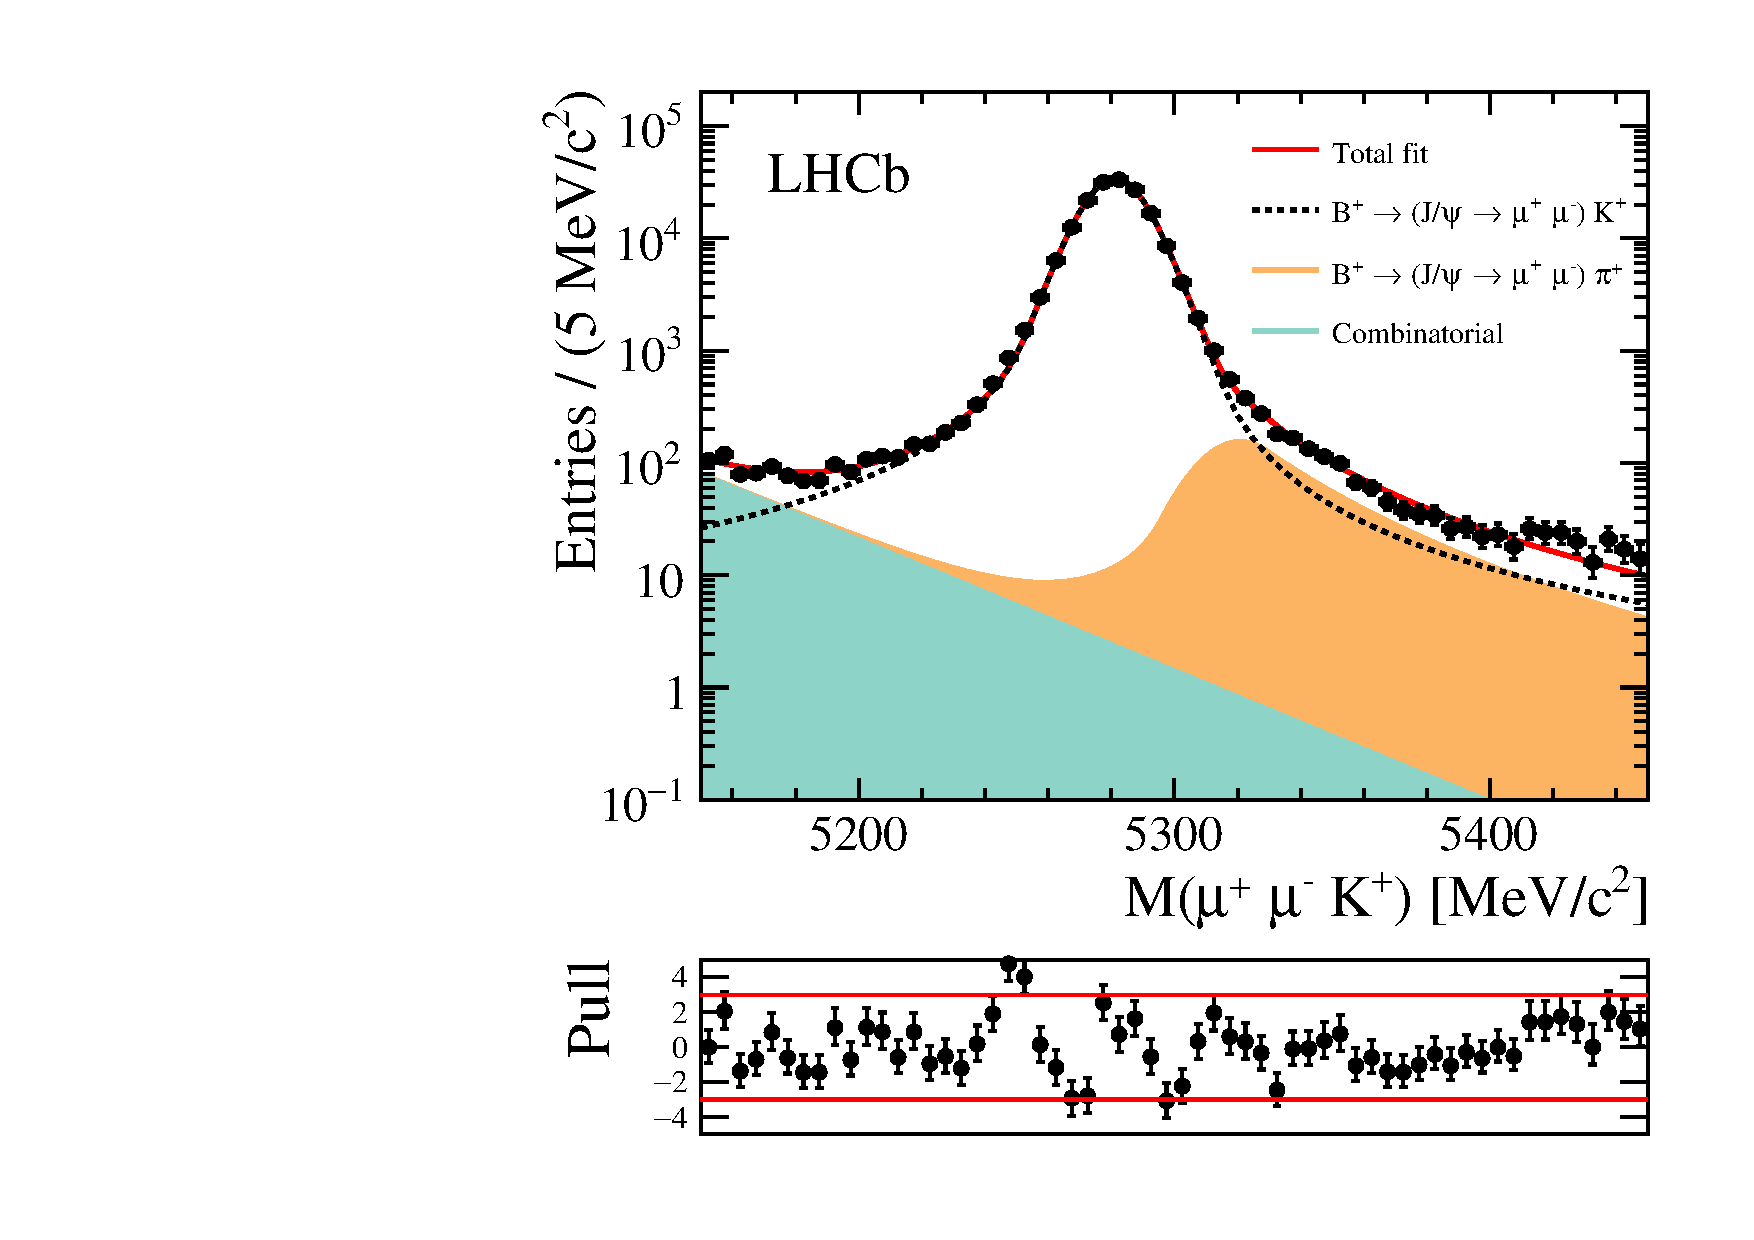
\includegraphics[width=0.5\linewidth]{./efficiency/controlchannelfits/controlnofcmeRun1.pdf}\put(-50,133){(a)}%
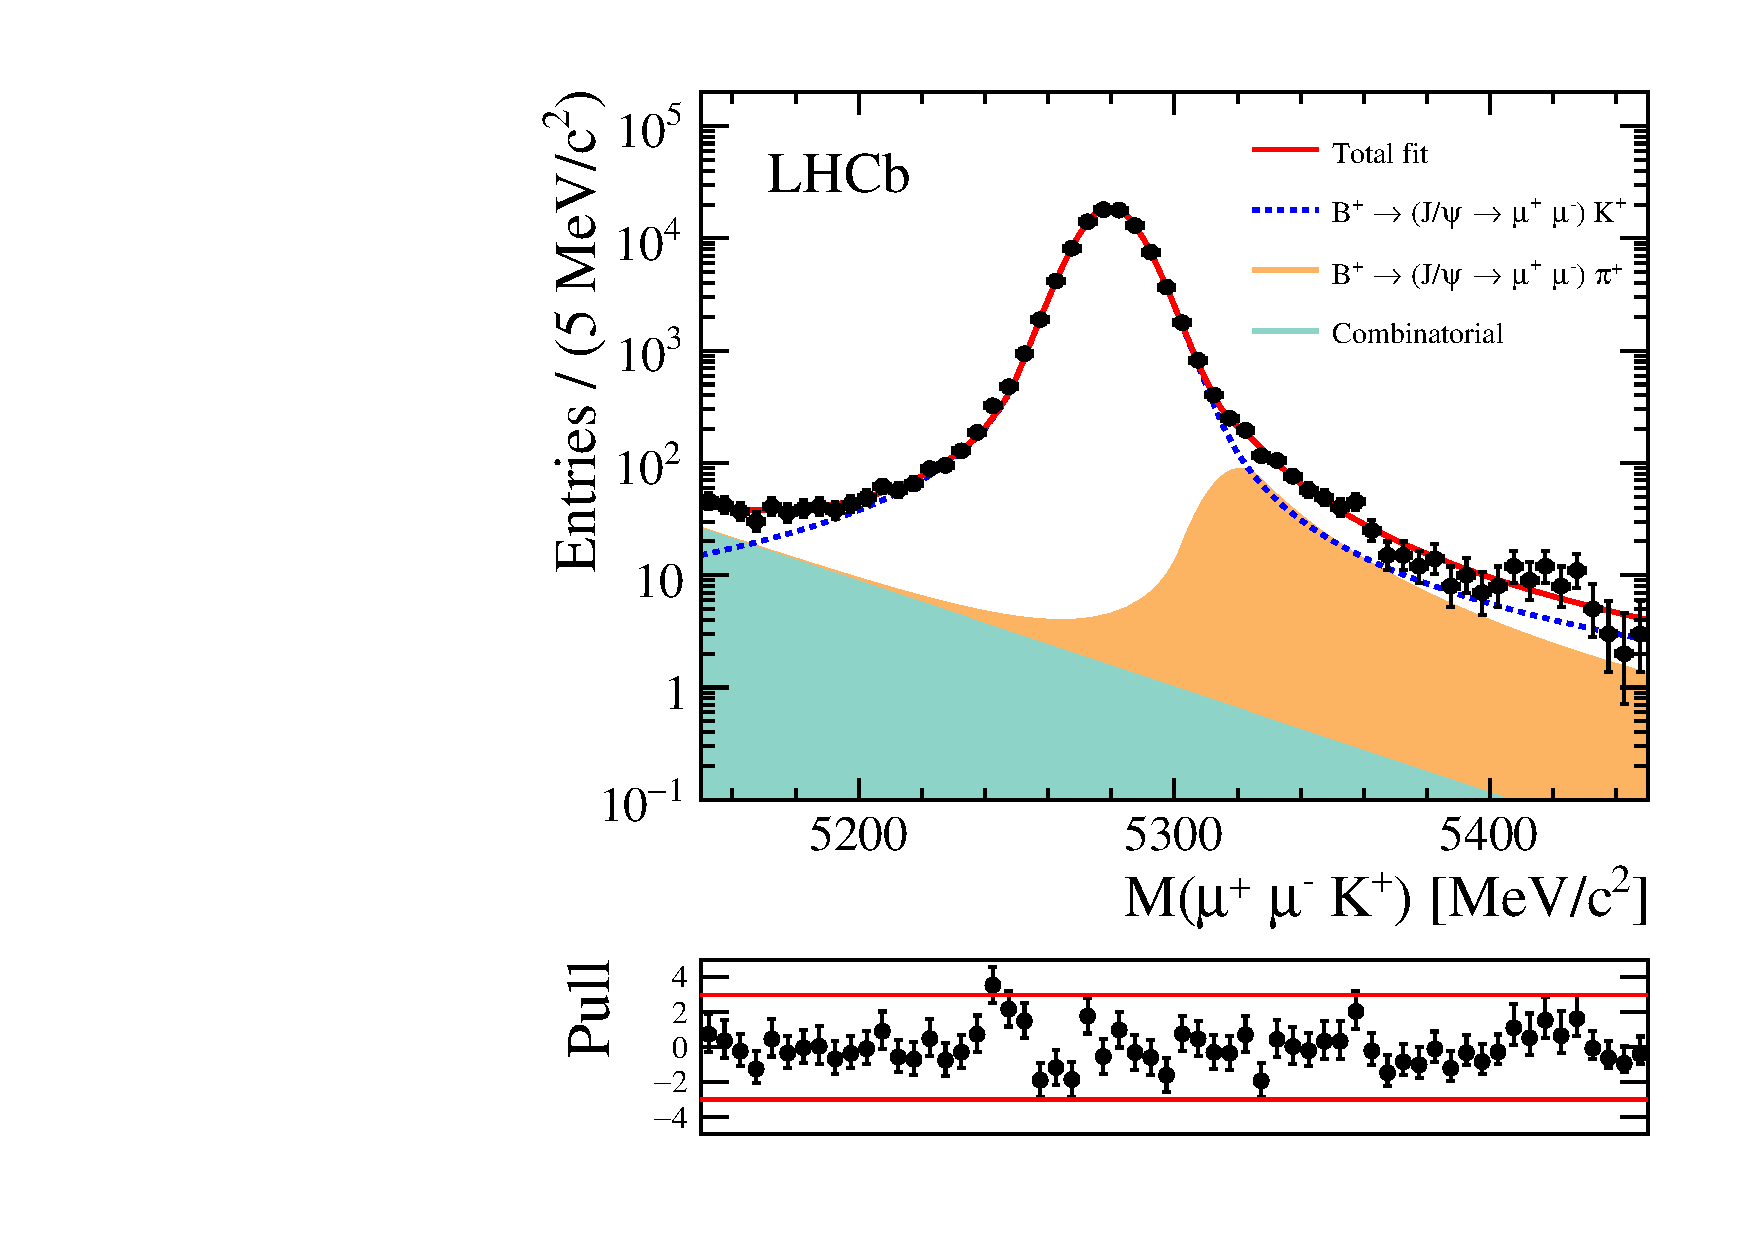
\includegraphics[width=0.5\linewidth]{./efficiency/controlchannelfits/controlnofcme2016.pdf}\put(-50,133){(b)}%

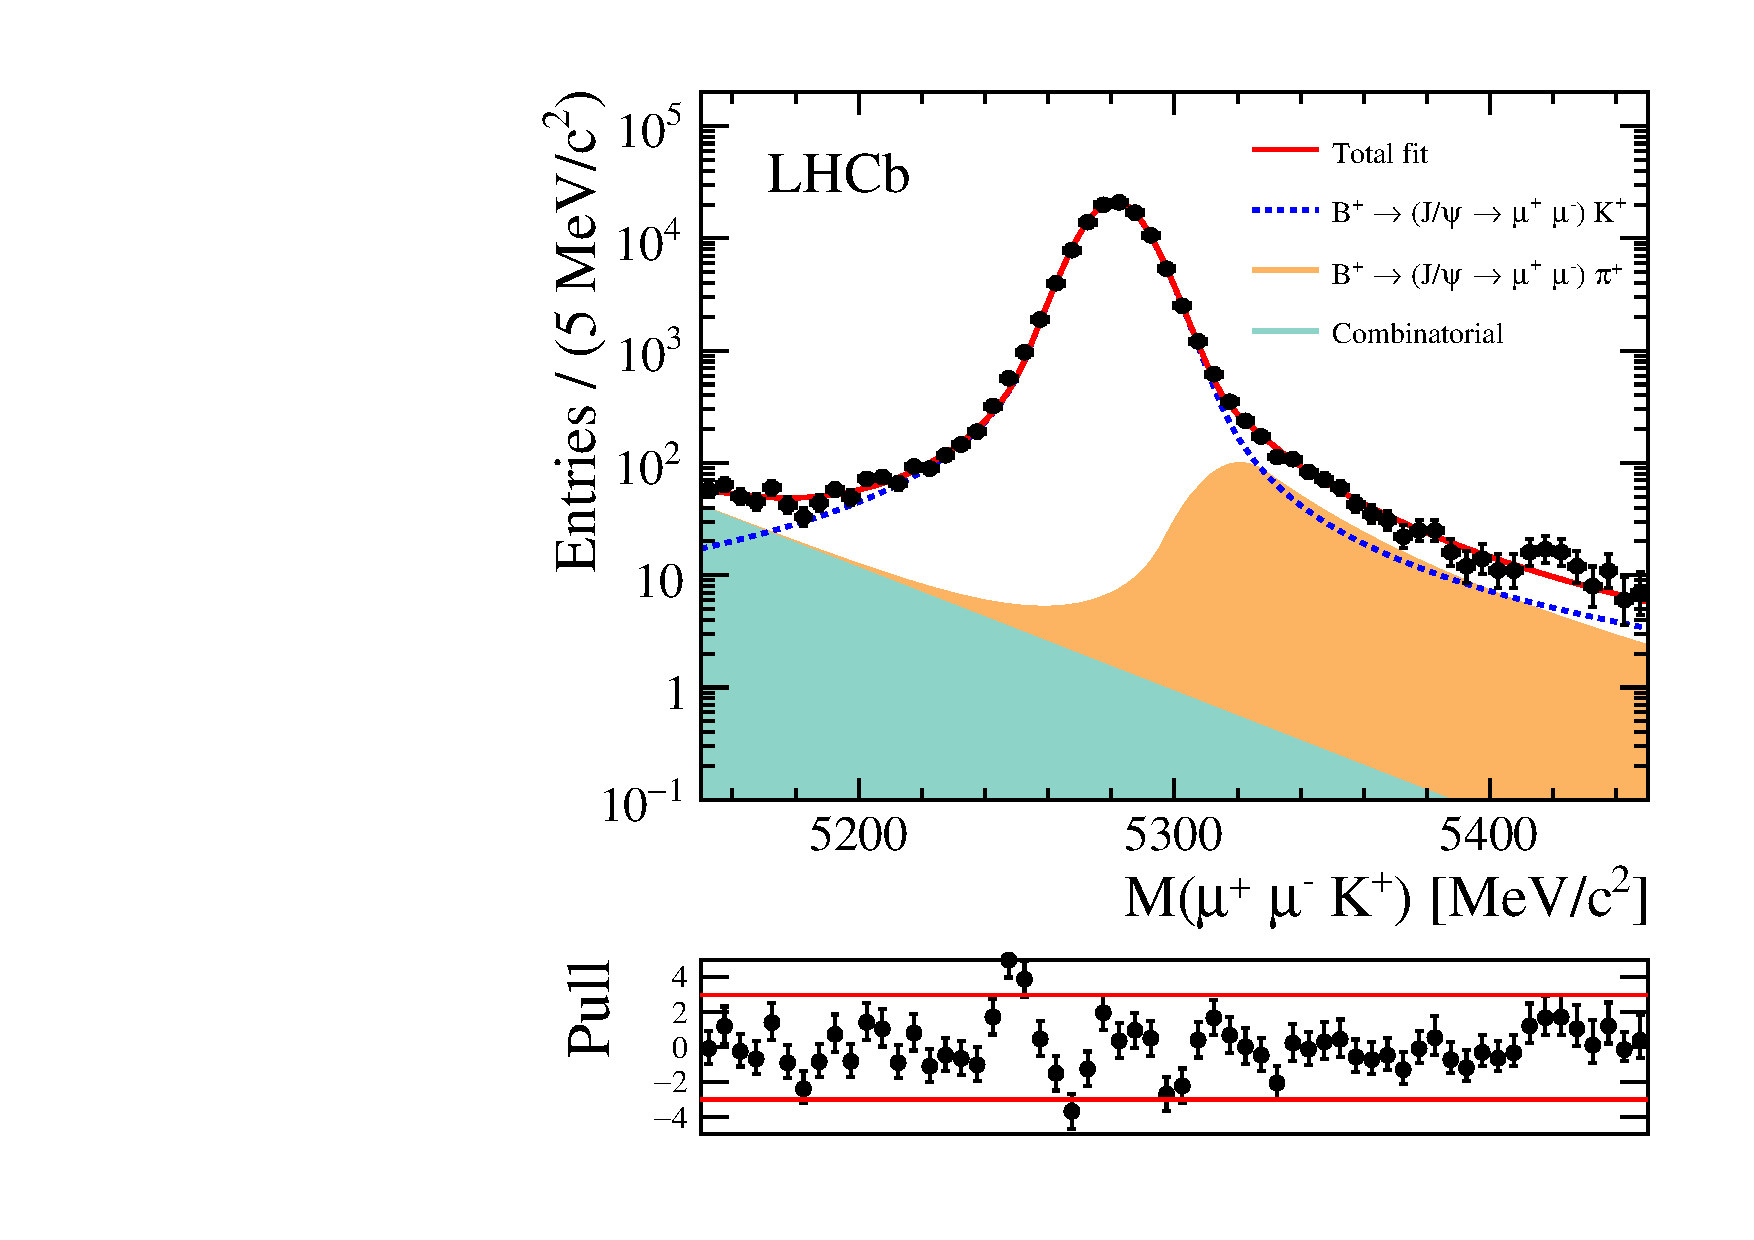
\includegraphics[width=0.5\linewidth]{./efficiency/controlchannelfits/controllowhfcmeRun1.pdf}\put(-50,133){(c)}%
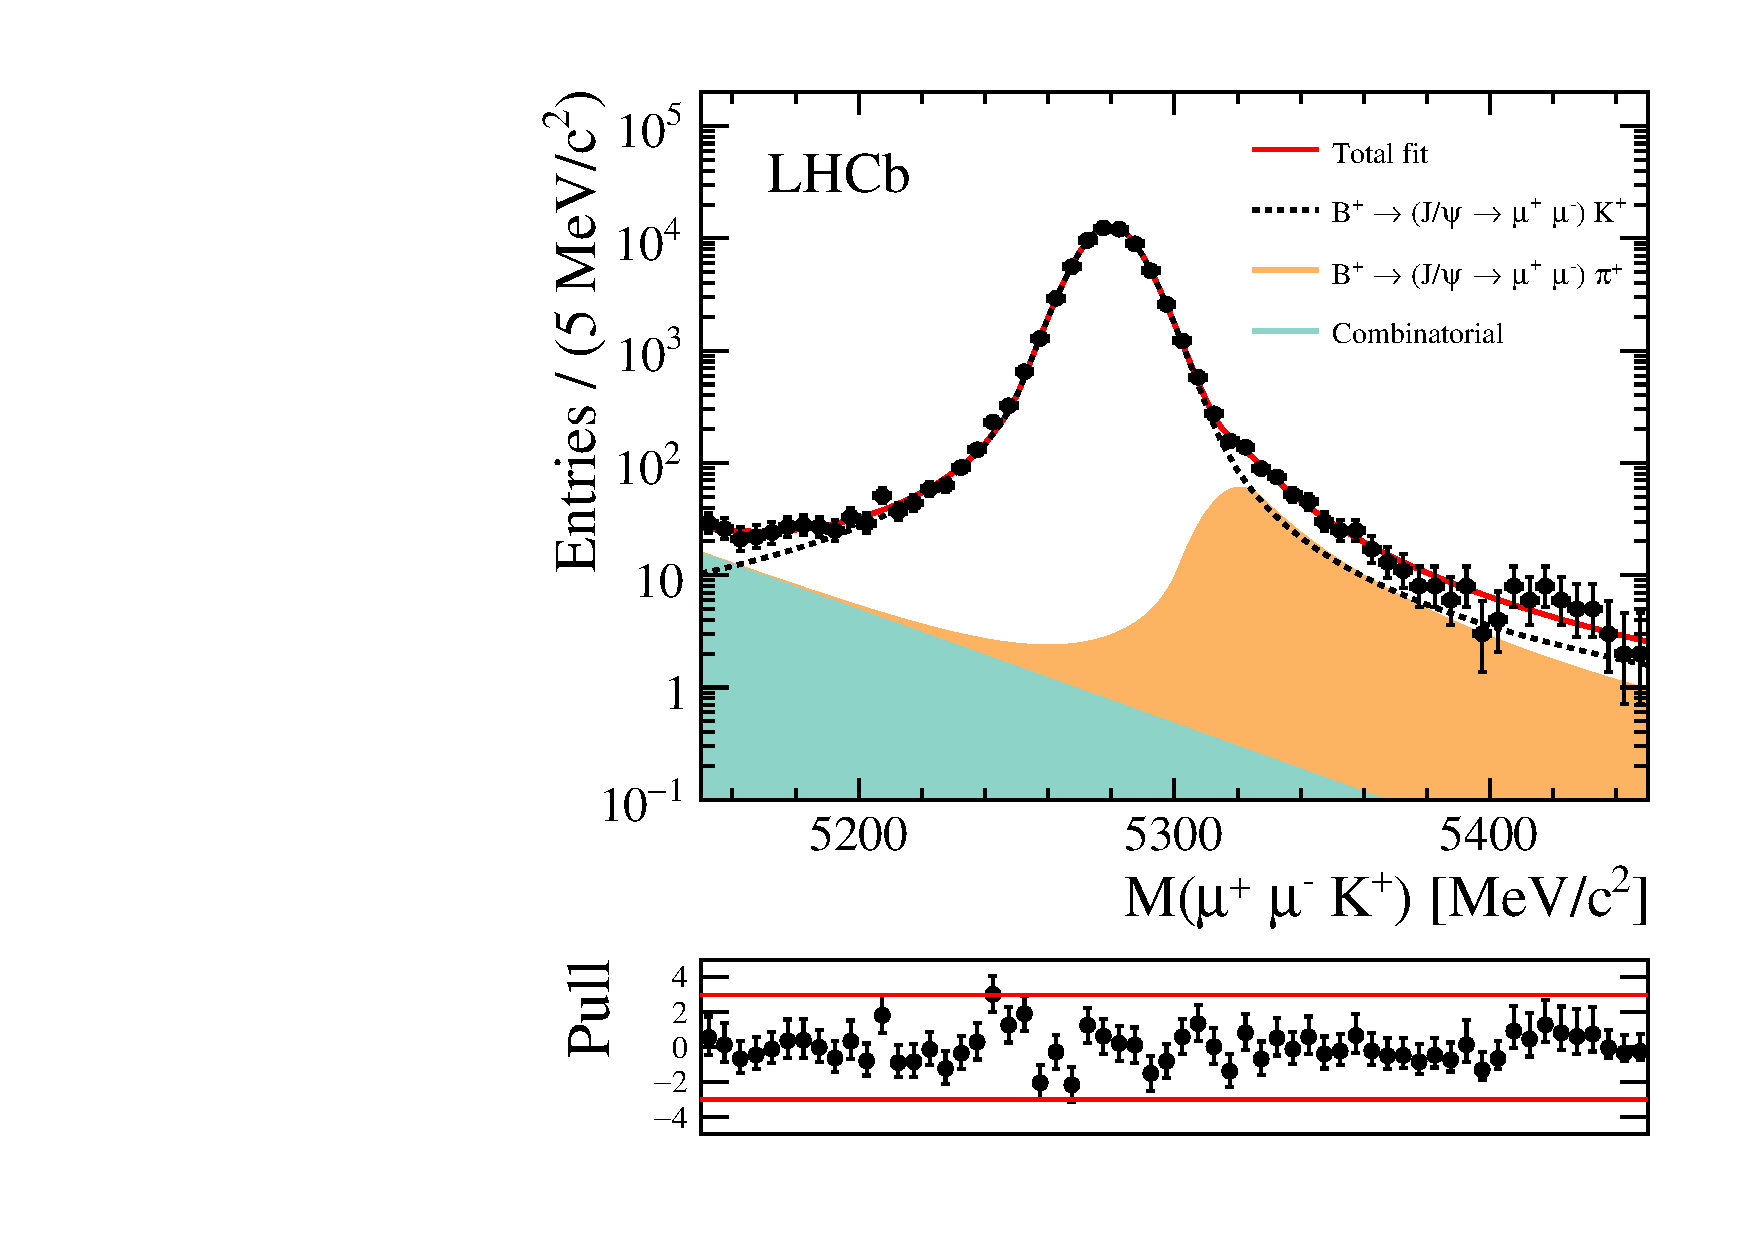
\includegraphics[width=0.5\linewidth]{./efficiency/controlchannelfits/controllowfcme2016.pdf}\put(-50,133){(d)}%


	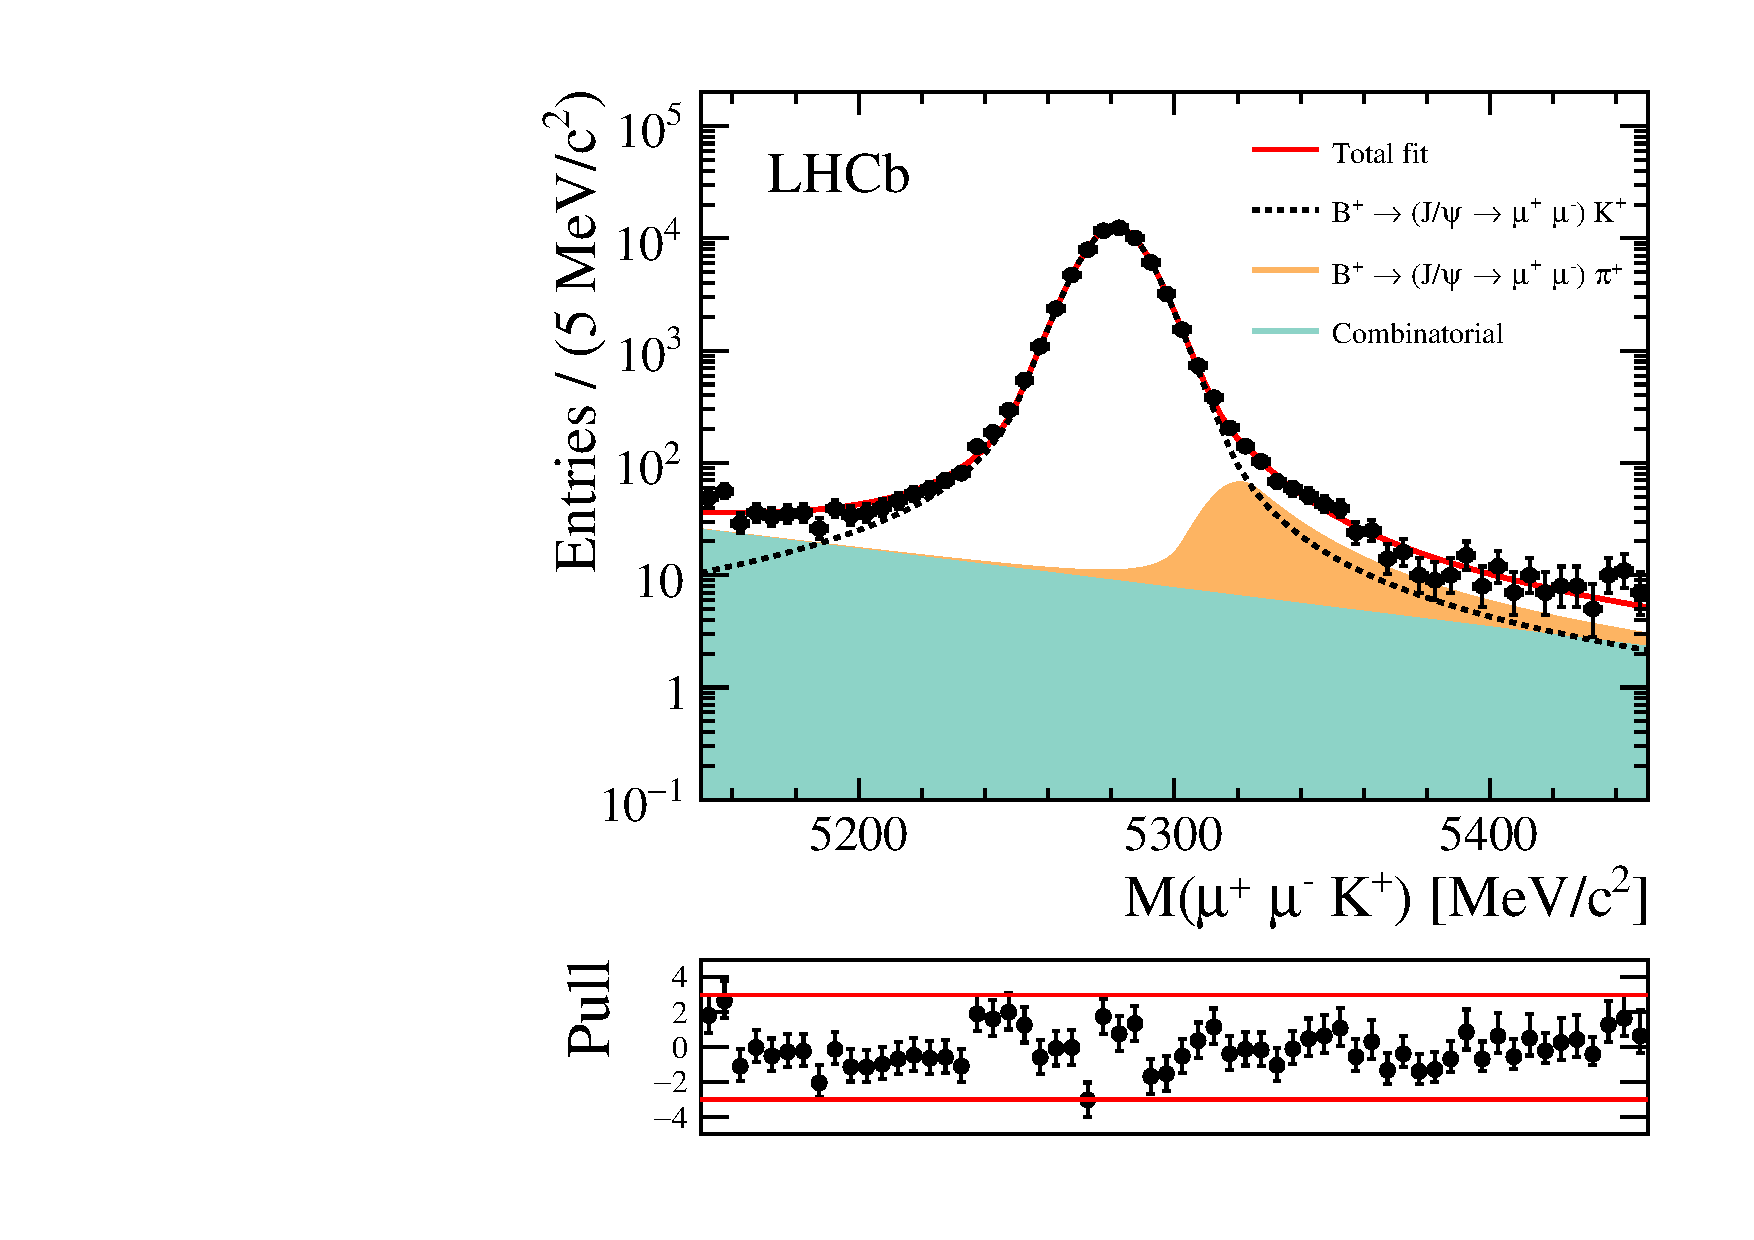
\includegraphics[width=0.5\linewidth]{./efficiency/controlchannelfits/controlhighfcmeRun1.pdf}\put(-50,133){(e)}%
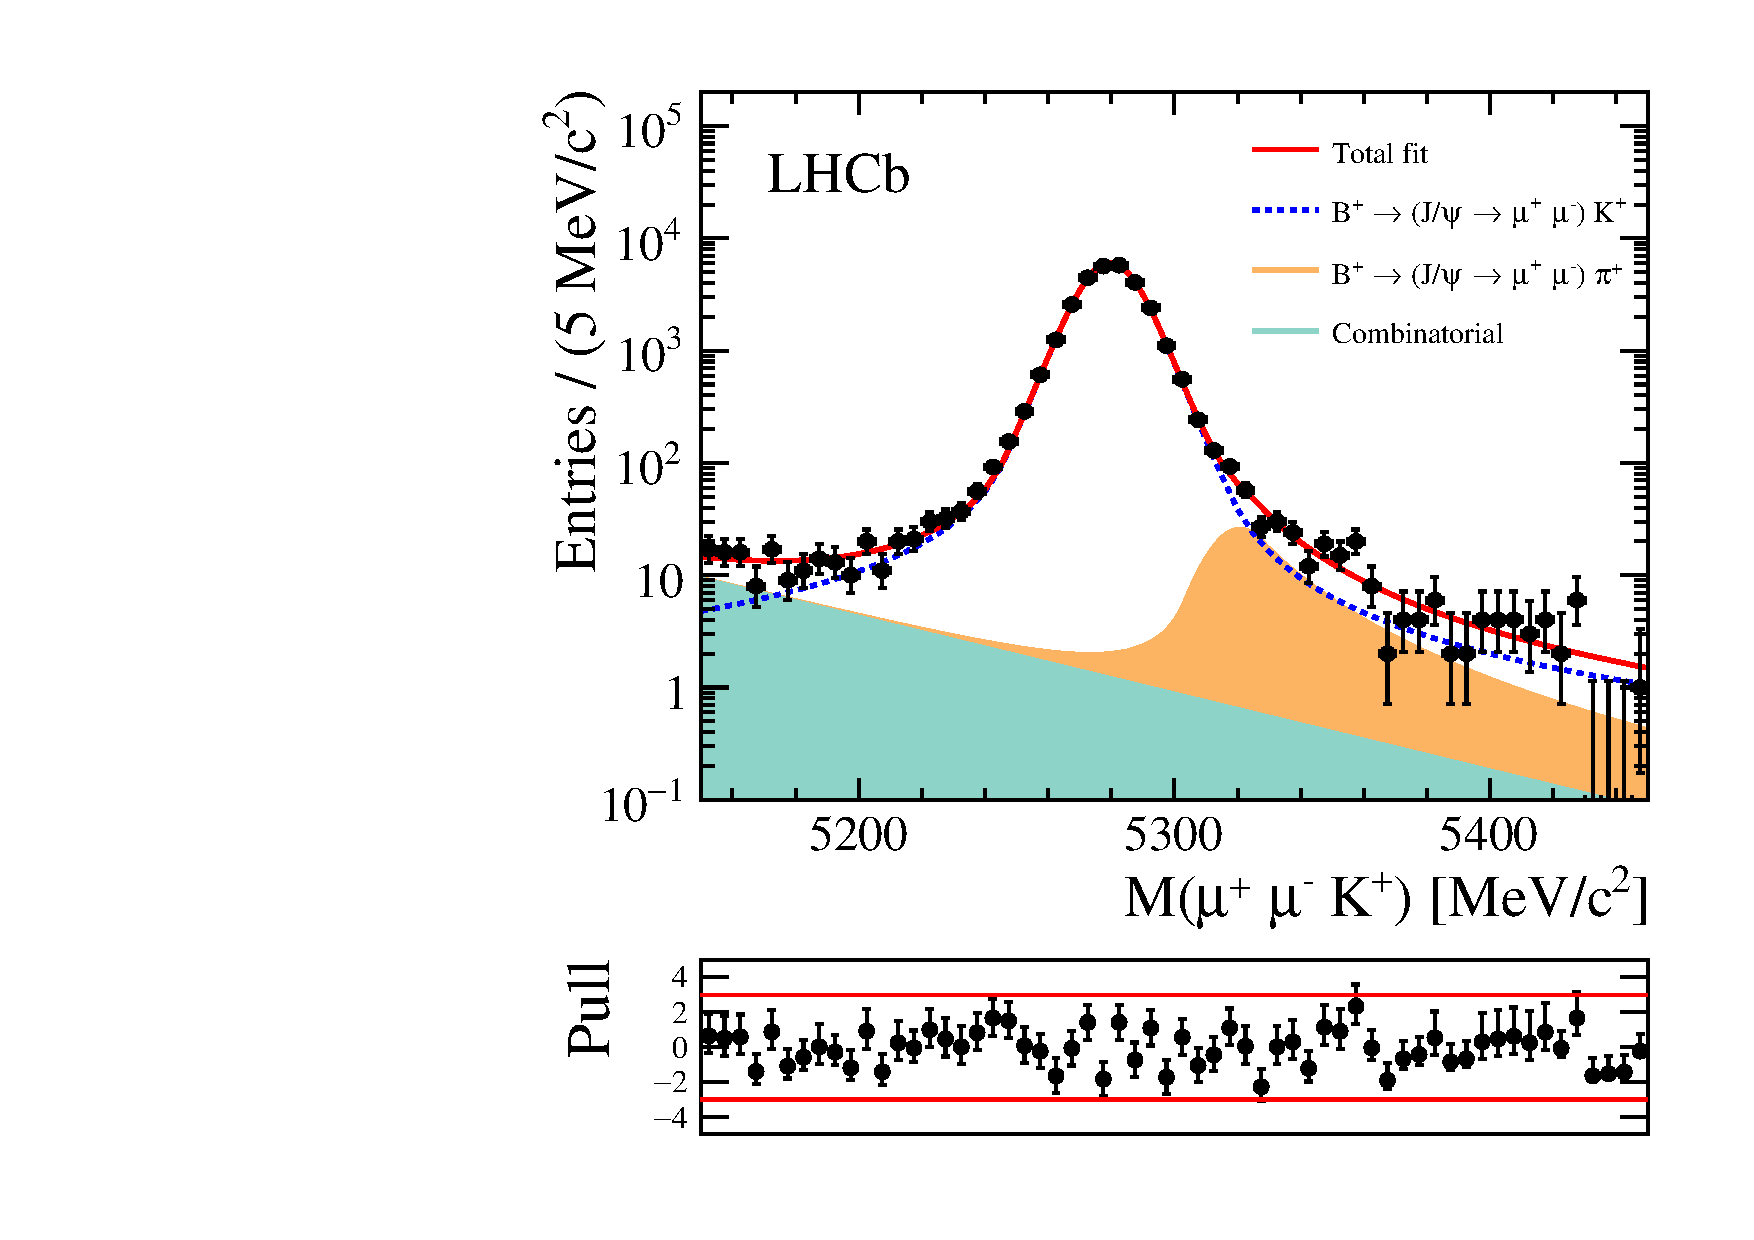
\includegraphics[width=0.5\linewidth]{./efficiency/controlchannelfits/controlhighfcme2016.pdf}\put(-50,133){(f)}%
%\includegraphics[width=0.5\linewidth]{./normalisationfits/HypatiaplotJpsiKFitLogyPrettyRun1lowFCME.pdf}\put(-50,133){(c)}%
%\includegraphics[width=0.5\linewidth]{./normalisationfits/HypatiaplotJpsiKFitLogyPretty2016lowFCME.pdf}\put(-50,133){(d)}%

%\includegraphics[width=0.5\linewidth]{./normalisationfits/HypatiaplotJpsiKFitLogyPrettyRun1highFCME.pdf}\put(-50,133){(e)}%
%\includegraphics[width=0.5\linewidth]{./normalisationfits/HypatiaplotJpsiKFitLogyPretty2016highFCME.pdf}\put(-50,133){(f)}%
\caption{Fit to (a) Stripping21 and 21r1 (b) Stripping 26 data with no fractional corrected mass split, (c)(d) low FCME, (e)(f)high FCME.}
%\vspace*{-1.0cm}
\label{fig:run1jpsikfitnofcme}
\end{figure}




Yields from fit to \bjpsimumuk are obtained and summarized in~\autoref{tab:normchannelyields}.
\begin{table}[H]
\begin{center}
\begin{tabular}{ l  l  l  l }
\toprule
Sample & Stripping & Split  &Yields \\
\midrule
	$N_{B^{+} \rightarrow J/\psi K^{+}}$  & Run \Rn{1} & NOFCME & 173422$\pm$446  \\
	$N_{B^{+} \rightarrow J/\psi K^{+}}$  & Run \Rn{2} & NOFCME &94491$\pm$313  \\
\midrule
$N_{B^{+} \rightarrow J/\psi K^{+}}$  & Run \Rn{1} & lowFCME & 109224$\pm$337  \\
$N_{B^{+} \rightarrow J/\psi K^{+}}$  & Run \Rn{2} & lowFCME & 64723$\pm$259  \\
\midrule
$N_{B^{+} \rightarrow J/\psi K^{+}}$  & Run \Rn{1} & highFCME &64078$\pm$257  \\
$N_{B^{+} \rightarrow J/\psi K^{+}}$  & Run \Rn{2} & highFCME & 29760$\pm$176  \\
\bottomrule
\end{tabular}
\end{center}
	\caption{ \bjpsimumuk signal yield obtained from fits to $\mu^{+} \mu^{-} K^{+}$ mass spectrum shown in~\autoref{fig:run1jpsikfitnofcme}.}
\label{tab:normchannelyields}
\end{table}




\subsection{Signal Fit}


\section{Efficiency Ratio}
\label{EfficiencyRatio}

As this measurement is performed in a particular min$q^{2}$ region, discussed in ~\autoref{qsqchoice}, all signal efficiencies are calculated with the min$q^{2}$ selection imposed. 
Overall selection efficiency for signal, $\varepsilon^{s}$, and normalisation, $\varepsilon^{n}$, includes contributions from the detector acceptance efficiency labelled (GEN); the reconstruction selection efficiency (REC); the offline selection efficiency comprising of trigger (TRG), $J/\psi$ and $\Psi(2S)$ veto (OFF), MVA based selection efficiency (CombiBDT and MisidBDT); fitting region selection efficiency (FR); the efficiency of the PID requirement (PID). The summary of method used to extract signal efficiency is shown in Table ~\autoref{tab:signaleffsummary}. For normalisation channel, there is no $minq^2$ region selection and hence full (\textit{generator-level+detector}) simulation is used everywhere apart from $\varepsilon_{GEN}$, \textit{generator-level}.

\begin{table}[H]
\centering
\small
\hspace*{-0.5cm}\begin{tabular}{| l | l | l |}
\hline
Component & Method  \\ \hline
	$\varepsilon_{GEN}$, $\varepsilon_{REC}$ & \Rn{1}  \\
	$\varepsilon_{TRG}$, $\varepsilon_{OFF}$, $\varepsilon_{BDTs}$, $\varepsilon_{FR}$  & \Rn{2} \\
	$\varepsilon_{PID}$ & \Rn{3} \\
\hline
 \end{tabular}
 \caption{Method of obtaining efficiencies. Most of these efficiencies are evaluated using simulation, however, TRG and PID efficiencies are evaluted using data and/or simulation techniques.}
\label{tab:signaleffsummary}
\end{table}

The three methods for signal efficiency determination are listed:

\begin{itemize}
	\item Method \Rn{1} - The first two efficiencies, $\varepsilon_{GEN}$, $\varepsilon_{REC}$, for signal are obtained using privately generated simulation from \autoref{tab:MCPPass} using

\begin{equation}
{\varepsilon_{GEN,minq^{2}}}\times {\varepsilon_{REC,minq^{2}}}= \frac{N_{in\_acc,minq^{2}}}{N_{generated,minq^{2}}}\times \frac{N_{REC,minq^{2}}}{N_{in\_acc,minq^{2}}},
\end{equation}

\begin{equation}
N_{in\_acc,minq^{2}} = N_{in\_acc} \times \varepsilon_{minq^{2}}.
\label{eq:number}
\end{equation}

In Equation ~\autoref{eq:number}, $\varepsilon_{minq^{2}}$ is obtained by dividing number of generated events in \textit{generator-level} simulation (mentioned in \autoref{tab:MCPPass}) with minq$^2$ condition imposed, $N_{generated,minq^{2}}$, to total number of generated events, $N_{generated}$. $N_{in\_acc}$ is the number of events in \textit{generator-level+detector} simulation before reconstruction, $N_{REC,minq^{2}}$ is the number of events after reconstruction with minq$^2$ condition.
\item Method \Rn{2} - Divide number of events that passed the selection by total number of events prior to this particular selection step.
\item Method \Rn{3} - Data-driven approach using \texttt{PIDCalib} package explained in~\autoref{simulationchap} of determining PID efficiency is used.
\end{itemize}

Having all the individual efficiencies the relative efficiency with no FCME split, $R_{\rm{NOFCME}}^{\{21,26\}}(\varepsilon)$, can be calculated 

%\hspace*{-1.0cm}\begin{equation}
%R^{\{21,26\}}_{\{NOFCME\}}(\varepsilon)=\frac{\varepsilon^{s}}{\varepsilon^{n}}=\frac{\varepsilon_{GEN}^{s}}{\varepsilon_{GEN}^{n}} \times \frac{\varepsilon_{REC}^{s}}{\varepsilon_{REC}^{n}} \times \frac{\varepsilon_{TRG}^{s}}{\varepsilon_{TRG}^{n}} \times \frac{\varepsilon_{OFF}^{s}}{\varepsilon_{OFF}^{n}} \times \frac{\varepsilon_{CombiBDT}^{s}}{\varepsilon_{CombiBDT}^{n}} \times \frac{\varepsilon_{MisidBDT}^{s}}{\varepsilon_{MisidBDT}^{n}} \times \frac{\varepsilon_{fitrange}^{s}}{\varepsilon_{fitrange}^{n}} \times \frac{\varepsilon_{PID}^{s}}{\varepsilon_{PID}^{n}},
%\label{eq:notsplitted}
%\end{equation}

\hspace*{-1.0cm}\begin{equation}
	R_{\rm{NOFCME}}^{\{21,26\}}(\varepsilon)=\frac{\varepsilon^{s}}{\varepsilon^{n}}=\frac{\varepsilon_{GEN}^{s}}{\varepsilon_{GEN}^{n}} \times \frac{\varepsilon_{REC}^{s}}{\varepsilon_{REC}^{n}} \times \frac{\varepsilon_{TRG}^{s}}{\varepsilon_{TRG}^{n}} \times \frac{\varepsilon_{OFF}^{s}}{\varepsilon_{OFF}^{n}} \times \frac{\varepsilon_{CombiBDT}^{s}}{\varepsilon_{CombiBDT}^{n}} \times \frac{\varepsilon_{MisidBDT}^{s}}{\varepsilon_{MisidBDT}^{n}} \times \frac{\varepsilon_{FR}^{s}}{\varepsilon_{FR}^{n}} \times \frac{\varepsilon_{PID}^{s}}{\varepsilon_{PID}^{n}},
\label{eq:notsplitted}
\end{equation}

%\hspace*{-1.0cm}\begin{equation}
%\hspace*{-2.0cm}R^{\{21,26\}}_{\{lowFCME,highFCME\}}(\varepsilon)=\frac{\varepsilon^{s}}{\varepsilon^{n}}=\frac{\varepsilon_{GEN}^{s}}{\varepsilon_{GEN}^{n}} \times \frac{\varepsilon_{REC}^{s}}{\varepsilon_{REC}^{n}} \times \frac{\varepsilon_{TRG}^{s}}{\varepsilon_{TRG}^{n}} \times \frac{\varepsilon_{OFF}^{s}}{\varepsilon_{OFF}^{n}} \times \frac{\varepsilon_{CombiBDT}^{s}}{\varepsilon_{CombiBDT}^{n}} \times \frac{\varepsilon_{MisidBDT}^{s}}{\varepsilon_{MisidBDT}^{n}} \times \frac{\varepsilon_{fitrange}^{s}}{\varepsilon_{fitrange}^{n}} \ \frac{\varepsilon_{FCME}^{s}}{\varepsilon_{FCME}^{n}} \times \frac{\varepsilon_{PID}^{s}}{\varepsilon_{PID}^{n}},
%\label{eq:splitted}
%\end{equation}

%where NOFCME means one bin of fractional corrected mass error, lowFCME and highFCME fractional corrected mass error are two bins of fractional corrected mass error, see Section ~\ref{split} for more details. 

 where 21, 26 denote the stripping version for Run \Rn{1} and Run \Rn{2}.
%As seen in equations ~\ref{eq:notsplitted} and ~\ref{eq:splitted}, absolute selection efficiencies $\varepsilon^{s}$, $\varepsilon^{n}$ have several components.
%\newline Overall selection efficiency includes contribution from the detector acceptance efficiency labelled (GEN);
%the reconstruction selection efficiency (REC); the efficiency of the offline selection (OFF) comprising of trigger, $J/\psi$ and $\Psi(2S)$ veto, MVA based selection (CombiBDT and MisidBDT); fitting region selection (fitrange); the efficiency of the PID requirement (PID). Individual  

%Since this analysis will be perfomed in two bins of FCME, and in two Stripping version there will be 4 efficiency ratios.  Most of these efficiencies are evaluated using MC, however, TRG and PID efficiencies will be evaluted using data and/or MC techniques. Values for different efficiencies and exact method of obtaining them is described in the following subsections.


\section{Summary of Efficiencies}
\label{EfficiencySummary}

The summary of individual efficiencies together with total efficiency, which is calculated for signal using nominator of \autoref{eq:notsplitted} and for normalisation denominator of \autoref{eq:notsplitted}, is given in \autoref{tab:effsumarry}.
%taken from /vols/lhcb/ss4314/tablesforana/efficiencyratios/2016/SesFUMSB_NOTsimultaneous_full_Error/plot_interesting/bin/*OK*per*tex
\begin{table}[H]
\begin{center}
\medskip
\begin{tabular}{ 
  l|  
  >{\collectcell\num}r<{\endcollectcell}@{${}\pm{}$}>{\collectcell\num}l<{\endcollectcell} 
  >{\collectcell\num}r<{\endcollectcell}@{${}\pm{}$}>{\collectcell\num}l<{\endcollectcell} |
  >{\collectcell\num}r<{\endcollectcell}@{${}\pm{}$}>{\collectcell\num}l<{\endcollectcell}
  >{\collectcell\num}r<{\endcollectcell}@{${}\pm{}$}>{\collectcell\num}l<{\endcollectcell}
  }	
%\toprule


        \hline
\multicolumn{1}{l|}{} & \multicolumn{4}{c|}{$ B^{+} \rightarrow \mu^{+} \mu^{-} \mu^{+} \nu$} & \multicolumn{4}{c}{$B^{+} \rightarrow (J/\psi \rightarrow \mu^{+} \mu^{-}) K^{+}$} \\
	Efficiency & \multicolumn{2}{c}{2012} & \multicolumn{2}{c|}{2016} & \multicolumn{2}{c}{2012} & \multicolumn{2}{c}{2016} \\

%\midrule

        \hline

$\varepsilon_{GEN}$ & 18.56& 0.11 & 19.59& 0.07 & 16.22& 0.02 & 17.39& 0.02 \\
$\varepsilon_{REC}$ & 10.84& 0.03 & 12.40& 0.01 & 17.74& 0.01 & 20.03& 0.00 \\
$\varepsilon_{TRG}$ & 74.22& 0.13 & 74.83& 0.05 & 77.79& 0.03 & 79.12& 0.01 \\
$\varepsilon_{OFF}$ & 88.20& 0.11 & 88.30& 0.05 & 100.00& 0.00 & 100.00& 0.00 \\
$\varepsilon_{CombiBDT}$ & 47.25& 0.18 & 34.28& 0.07 & 50.89& 0.05 & 39.73& 0.02 \\
$\varepsilon_{MisidBDT}$ & 43.58& 0.26 & 36.80& 0.12 & 51.12& 0.07 & 44.64& 0.02 \\
$\varepsilon_{FR}$ & 92.30& 0.21 & 93.77& 0.10 & 99.59& 0.01 & 99.91& 0.00 \\
$\varepsilon_{PID}$ & 63.15& 0.50 & 62.27& 0.27 & 68.53& 0.11 & 65.63& 0.04 \\
\hline

$\varepsilon_{total}$ & 0.1581& 0.0020 & 0.1182& 0.0008 & 0.3974& 0.0011 & 0.3203& 0.0005 \\

	
	
	\hline
%\bottomrule
\end{tabular}
\end{center}
	\caption{Summary of individual simulation and/or data efficiencies in \% necessary for \textit{single event sensitivity} for signal and normalisation channel. Efficiency values for 2016 are TCK-weighted averaged efficiencies, which will be explained in \autoref{trigef}. The errors considered are of statistical nature, computed using binomial error.}
\label{tab:effsumarry}
\end{table}


Hence resulting values for relative no fractional corrected mass split efficiency ratios defined in \autoref{eq:notsplitted} are

\begin{equation}
	R^{21}_{\rm{NOFCME}}(\varepsilon)=\frac{(1.58\pm0.02)\times 10 ^{-3 }}{(3.97\pm0.01)\times 10 ^{-3 }}=(3.98\pm0.05)\times 10 ^{-1 },
\end{equation}

\begin{equation}
	R^{26}_{\rm{NOFCME}}(\varepsilon)=\frac{(1.18\pm0.01)\times 10 ^{-3 }}{(3.20\pm0.00)\times 10 ^{-3 }}=(3.69\pm0.03)\times 10 ^{-1 }.
\end{equation}


Including fractional corrected mass split efficiency ratios defined in~\autoref{eq:impsplit} are

\begin{equation}
	R^{21}_{\rm{lowFCME}}(\varepsilon)=\frac{(7.44\pm0.12)\times 10 ^{-4 }}{(2.33\pm0.01)\times 10 ^{-3 }}=(3.20\pm0.05)\times 10 ^{-1 },
\end{equation}
\begin{equation}
	R^{21}_{\rm{highFCME}}(\varepsilon)=\frac{(8.37\pm0.13)\times 10 ^{-4 }}{(1.65\pm0.01)\times 10 ^{-3 }}=(5.09\pm0.08)\times 10 ^{-1 },
\end{equation}

\begin{equation}
	R^{26}_{\rm{lowFCME}}(\varepsilon)=\frac{(6.51\pm0.05)\times 10 ^{-4 }}{(2.15\pm0.00)\times 10 ^{-3 }}=(3.03\pm0.02)\times 10 ^{-1 },
\end{equation}
\begin{equation}
	R^{26}_{\rm{highFCME}}(\varepsilon)=\frac{(5.33\pm0.05)\times 10 ^{-4 }}{(1.05\pm0.00)\times 10 ^{-3 }}=(5.06\pm0.04)\times 10 ^{-1 }.
\end{equation}
	
	
As it can be noticed, different selections that were optimised for Run \Rn{1} and \Rn{2} yield different overall as well as individual efficiencies. This results in small differences in sensitivity between Run \Rn{1} and Run \Rn{2}. To better understand where does this difference come from, ratio of individual relative efficiencies as a function of stripping version is plotted in the~\autoref{fig:rateffsnofcme}. The difference can be attributed to different BDTs.

\begin{figure}[H]
\centering
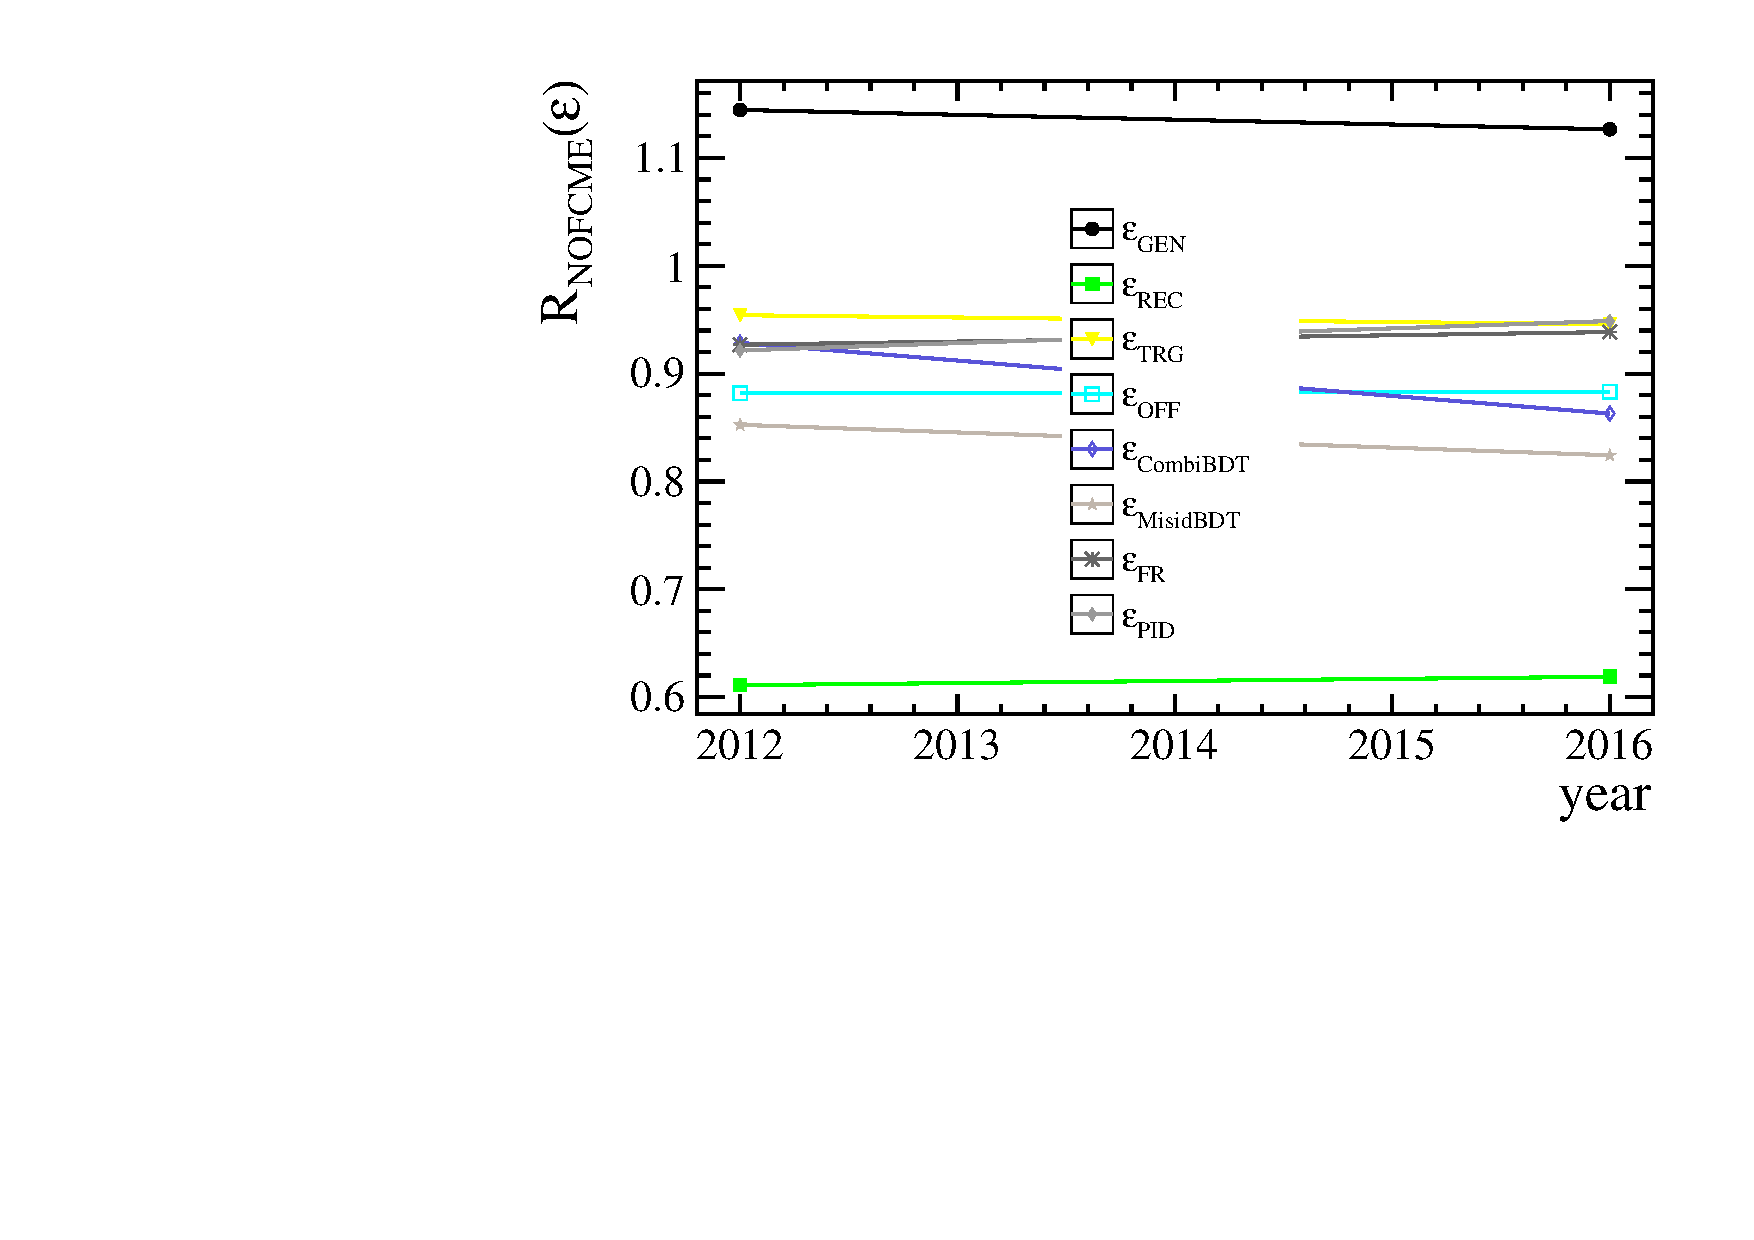
\includegraphics[width = 0.8\textwidth]{efficiency/effiratio/Plot_ALL_Efficiencies_Ratio_Overview_Pretty.pdf}
\caption{Summary of ratio of efficiencies between 2012 simulation and 2016 simulation with no FCME split. Efficiency values for 2016 are TCK-weighted averaged efficiencies.}
\centering
\label{fig:rateffsnofcme}
\end{figure}


More detailed discussion on individual efficiencies is covered in following subsections. 


\subsection{Detector Acceptance Efficiency (GEN)}
For charged particles detector acceptance efficiency describes the fraction of decays contained in the polar angle region of [10, 400] mrad.  
For 2012 and 2016 simulation samples, the overall detector acceptance efficiency will be the average for two possible magnetic polarity conditions: down, up. For 2012 this will be also averaged with two different simulation versions: Pythia 6.4\cite{pythia6} and Pythia 8.1\cite{pythia8}.

The hierarchy of generator level efficiencies $\varepsilon^{s}_{GEN} > \varepsilon^{n}_{GEN}$ is expected as the muon is lighter than kaon making kaon more likely to be softer and at larger angle, therefore outside of the acceptance. 

%
%        \begin{table}[H]
%                \begin{center}
%        \begin{tabular}{l c c }
%
%%        \hline
%                Channel & Year & $\varepsilon_{gen}$\\ \hline
%              %  $B^{+} \rightarrow J/\psi K^{+}$ & 2011 &  Sim08, Pyth6 & N/A & N/A & \\
%              %  $B^{+} \rightarrow J/\psi K^{+}$ & 2011 &  Sim08, Pyth8 & 0.16379 $\pm$ 0.00030 & 0.16366 $\pm$ 0.00030 & 0.16372$\pm$0.00021 \\
%                \Bmumumu & 2012 & 0.1856$\pm$0.0011 \\
%%                \Bmumumu & 2012 & \\
%                \Bmumumu & 2016 & 0.1959$\pm$0.0016 \\ \hline
%
%                \bjpsimumuk & 2012 & 0.1622$\pm$0.0002\\
%                %$B^{+} \rightarrow J/\psi K^{+}$ & 2012 &  \\
%                %$B^{+} \rightarrow J/\psi K^{+}$ & 2015 &  Sim09a, Pyth8 & 0.17304 $\pm$ 0.00048 & 0.17386 $\pm$ 0.00047 &0.17346$\pm$0.00034 \\
%                \bjpsimumuk & 2016 &  0.1739$\pm$0.0004  \\
%                \hline
%%               \Bmumumu & 2012 &  Sim08, Pyth6 &0.1828$\pm$0.0015 & \multirow{2}{*}{0.1856$\pm$0.0011} \\
%%                \Bmumumu & 2012 &  Sim08, Pyth8 &0.1884$\pm$0.0015 & \\
%%                \Bmumumu & 2016 &  Sim09b, Pyth8 &0.1959$\pm$0.0016 & 0.1959$\pm$0.0016 \\
%              %  $B^{+} \rightarrow J/\psi \pi^{+}$ & 2012 &  Sim08, Pyth6 & 0.1519 $\pm$ 0.000400 & N/A & \multirow{2}{*}{0.15816$\pm$0.00024}\\
%              %  $B^{+} \rightarrow J/\psi \pi^{+}$ & 2012 &  Sim08, Pyth8 & 0.1622 $\pm$ 0.000424 & 0.1611 $\pm$ 0.000421 &  \\
%%               \hline
%              %  $B^{0} \rightarrow J/\psi K^{*}$ & 2012 &  Sim08, Pyth8 & 0.16141 $\pm$ 0.00043 & 0.16050 $\pm$ 0.00043 &0.16095$\pm$0.00030 \\
%%                \hline
%              %  PartReco & 2012 & Sim08, Pyth8 & 0.16058 $\pm$ 0.00051 & 0.16058 $\pm$ 0.00050 & 0.1606$\pm$0.0004 \\
%%                \hline
%                \end{tabular}
%        \end{center}
%        \caption{Geometrical detector acceptance efficiencies for signal and normalisation channel. For 2012 and 2016 simulation samples, the overall detector acceptance efficiency will be the average for two possible magnetic polarity conditions: down, up. For 2012 this will be also averaged with two different simulation versions: Pythia 6.4\cite{pythia6} and Pythia 8.1\cite{pythia8}.}%  Efficiencies were calculated by generating statistics tables generated using dirac-bookeeping-prod4path, looking at generator level cut efficiency: /afs/cern.ch/user/s/slstefko/cmtuser/stattables.}
%        \label{tab:MCdeteff}
%        \end{table}

\subsection{Reconstruction Efficiency (REC)}
The reconstruction efficiency is calculated on simulated events which have passed the detector acceptance. For signal, this efficiency consists of reconstruction and stripping, detailed in~\autoref{tab:stripcutsB}. For normalisation it consists from reconstruction, stripping, \textbf{and on the top} signal stripping is applied. This is done so that selections in normalisation and signal channel are kept as similar as possible and the fact that the signal selection has tighter cuts as explained in \autoref{nchannel}. However, it should be noted that reconstruction efficiency reflects stripping selection \textbf{without the PID cuts} for both signal and normalisation. This is because \gls{PID} is badly modelled in simulation and hence will be accounted for separately and at the end of the selection chain.

The hierarchy of reconstruction level efficiencies $\varepsilon^{s}_{REC} < \varepsilon^{n}_{REC}$ is also expected as many variables in a signal stripping are based on alignment of the mother $B$ with its daugthers. For fully reconstructed normalisation channel this is expected to be the case, whereas for not fully reconstructed decays alignment requiremnts make selection tighter. 

%  \begin{table}[H]
%                \begin{center}
%        \begin{tabular}{l c c }
%
%    %    \hline
%		Channel & Year & $\varepsilon_{rec|sel}$ \\ \hline
%                \Bmumumu & 2012 &  0.10841$\pm$0.00030 \\
%                \Bmumumu & 2016 &  0.12417$\pm$0.00032 \\ \hline
%                \bjpsimumuk & 2012 & 0.17741$\pm$0.00013 \\ \
%%$B^{+} \rightarrow J/\psi K^{+}$ & 2015 &  Sim09a, Pyth8 & 4201997 & & \\
%                \bjpsimumuk & 2016 &  0.20031$\pm$0.00011 \\
%		
%		\hline
%        \end{tabular}
%        \end{center}
%        \caption{Reconstruction and preselection efficiencies for signal and normalisation channels.}
%        \label{tab:myreco}
%        \end{table}


\subsection{Trigger Efficiency (TRG)}
\label{trigef}
 The trigger efficiency is calculated on the top of (GEN) and (REC) efficiency. In order to extract the trigger efficiency, full simulation for both signal and normalisation is used. It should be noted though that at \gls{LHCb}, full simulation is produced based on a certain trigger configuration. Trigger configuration key, TCK, represents unique code for exact conditions the data have been triggered with at \texttt{L0}, \texttt{HLT1} and \texttt{HLT2}, notably thresholds of certain quantities such as $p$, $p_{T}$. 
 
Therefore if default TCK for simulation is representative for the whole considered dataset then the efficiency can be extracted directly from the simulation produced, which is the case for the Run \Rn{1} data.

However in Run \Rn{2} the trigger thresholds have been changing often resulting in 16 different TCKs with very different $p$, $p_{T}$ thresholds, see Table ~\autoref{tab:2016MC} for full detail. In the third column, luminosity proportion for 2016 is given. It can be seen that the default simulation in 2016 (corresponding to TCK decimal key 288888335) only represents around 35\% of the data. For this reason, the trigger efficiencies for 2016 data have been obtained by emulation of the trigger on simulation for \texttt{L0} and \texttt{HLT1} level for each individual TCK, creating 16 TCK-based simulations.  This trigger emulation to extract efficiencies was tested with the default trigger configuation (TCK 288888335) to validate the emulation and the correct efficiencies have been recovered. It should be noted that small differences arise from difference between \textit{offline} and \texttt{HLT1} container for \gls{PV}s which stores the information about \gls{minipchi2} as the \gls{PV} finding-algorithm is different, but these have neglgible effect. \mybox{mentioning this jsut i case of reproducibility, but maybe not necessary}.
%Therefore the emulation will not be exact, however, the effect is very small as it seems to be only resolution that will slightly shift the distribution, see figure ~\autoref{fig:hlt1shortcoming} 

In order to obtain the average efficiency for Run \Rn{2}, the 16 TCK efficiencies are weighted by the proportion of luminosity corresponding to the integrated luminosity for a given TCK over the full 2016 integrated luminosity. The integrated luminosity per TCK was extracted by looking at API version of the LHCb rundatabase. 

The full trigger luminosity for Run \Rn{2} is calculated by averaging the luminosity-weighted efficiencies, as seen in ~\autoref{tab:L0andHLT1Calib}. This averaged efficiency is going to be given as a final efficiency for 2016 from now on.  


\begin{table}
	\begin{center}
\footnotesize
      \begin{tabular}{l l l l | l l l l | l l }
      \multicolumn{4}{c |}{ } & \multicolumn{4}{c|}{\texttt{HLT1TrackMuon}} & \multicolumn{2}{c}{\texttt{L0Muon}}\\ \hline
	      TCK dec & TCK hex & \%$\mathcal{L}$ & $\mathcal{L}$ & \gls{pgh2} & $p_{\mu}$ & $p_T(\mu)$ & \gls{minipchi2} & $SPD_{mult}$ & $p_T(\mu)$\\% & $sum_{ET}$\\
	      &  & \% & $\textrm{pb}^{-1}$ & & [\mev] & [\mev] &  & & [\mev] \\% & $sum_{ET}$\\
      \multicolumn{10}{c}{\textbf{2016 MD} $0.859656\,\textrm{fb}^{-1}$} \\
      287905280 & 0x11291600 & $0.769$ & $12.74$  & $-$ & 6.0 & 0.91 & 10        & 450  & 14 \\% &  $-$\\
      287905283 & 0x11291603 & $2.11$ & $35.01$  & $-$ & 6.0 & 0.91 & 10         & 450  & 23 \\% &  $-$ \\
      287905284 & 0x11291604 & $1.50$ &  $24.78$  & $-$ & 6.0 & 0.91 & 10        & 450  & 27 \\% & $-$ \\
      287905285 & 0x11291605 & $4.73$ &   $78.42$   & $-$ & 6.0 & 0.91 & 10      & 450 & 31 \\% & $-$ \\
      288822793 & 0x11371609 & $4.35$   &  $72.14$ & 0.2 & 6.0 & 1.1  & 35       & 450  & 27 \\% & $-$ \\
      288822798 & 0x1137160e & $1.37$  &  $22.756$ & 0.2 & 6.0 & 1.1  & 35       & 450  & 27 \\% & $-$ \\
      288888329 & 0x11381609 & $0.414$  &  $6.86$  & 0.2 & 6.0 & 1.1  & 35       & 450 & 31 \\% & $-$ \\
      288888334 & 0x1138160e & $1.912$  &  $31.70$  & 0.2 & 6.0 & 1.1  & 35      & 450 & 31 \\% & $-$ \\
      288888335 & 0x1138160f & $34.7$  &  $575.25$  & 0.2 & 6.0 & 1.1  & 35  & 450 & 37 \\% & $-$ \\
      \multicolumn{10}{c}{\textbf{2016 MU} $0.798156\,\textrm{fb}^{-1}$} \\
      288495113 & 0x11321609 & $6.45$ &  $107.00$   &  $-$ & 6.0 & 0.91 & 10 & 450 & 27 \\% & $-$   \\
      288626185 & 0x11341609 & $7.12$ &  $118.06$  &  $-$ & 6.0 & 0.91 & 10 & 450 & 27 \\% & $-$    \\
      288691721 & 0x11351609 &  $1.42$ &  $23.46$   &  0.2 & 6.0 & 1.1  & 35  & 450 & 27 \\% & $-$  \\
      288757257 & 0x11361609 & $25.0$ &  $414.62$   &  0.2 & 6.0 & 1.1  & 35 & 450 & 27  \\% & $-$   \\
      288888337 & 0x11381611 & $ 2.66$ &  $44.13$  &  0.2 & 6.0 & 1.1  & 35  & 450 & 31 \\% & $-$   \\
      288888338 & 0x11381612 & $5.41$ &  $89.75$  &  0.2 & 6.0 & 1.1  & 35  & 450 & 33 \\% & $-$    \\
      288888339 & 0x11381613 & $0.0685$ &  $1.136$  &  0.2 & 6.0 & 1.1  & 35  & 450 & 27 \\% & 1000 \\
      \multicolumn{10}{c}{\textbf{MC Default}} \\
      1362630159 & 0x5138160f & $-$  & $-$   & 0.2 & 6.0 & 1.1  & 35 & 450 & 37\\% &  157\\

   \end{tabular}
\caption{Summary of 16 different TCKs listing properties of candidates necessary to pass \texttt{L0} and \texttt{HLT1} selection in 2016. In the final row, the default configuration for 2016 is shown and it corresponds to 288888335 TCK.}
\label{tab:2016MC}
	\end{center}
\end{table}

For the \texttt{HLT2} level, there were no significant changes of thresholds and are hence efficiencies are obtained from full simulation regardless. The systematic effect of this assumption will be listed in the systematic uncertainties chapter \mybox{SALLY - ADD SECTION REFERENCE TO SYSTEMATICS}.




%As it can be seen in the list of trigger requirements in ~\ref{tab:triggersel}, \texttt{L0MuonDecision} needs to be modelled. This trigger line selects event candidates only if candidate has certain muon $p_{T}$ and $nSPD$ hits.


%\texttt{HLT1} trigger selection was also emulated offline as \texttt{HLT1}. The efficiency of \texttt{HLT1TrackMuonDecision} is then determined on the top of \texttt{L0MuonDecision} as only events which have passed either \texttt{L0MuonDecision} or \texttt{L0DimuonDecision} would be considered. \texttt{HLT1TrackMuonDecision} trigger lines requires events with only certain muon $p_{T}$,$p$, \textit{ghost probability} and $MIP\chi^{2}$. 

%There are other variables that are included in \texttt{HLT1TrackMuonDecision} such as whether the track is \gls{VELO} track or how many hits have been missed in \gls{VELO}, however, these have not changed throughout the Run \Rn{2} data and are not likely to be different between signal and normalisation channel.  Hence only efficiency for the relevant cuts are included in emulation of \texttt{HLT1TrackMuonDecision}.

%It should be noted that there is difference between \textit{offline} and \texttt{HLT1} container for PVs which stores the information about $MIP\chi^{2}$ fast Kalman fitter rather then full is used. Therefore the emulation will not be exact, however, the effect is very small as it seems to be only resolution that will slightly shift the distribution, see figure ~\autoref{fig:hlt1shortcoming}.

%This trigger emulation to extract efficiencies was tested with the default trigger configuation to validate the emulation and the correct efficiencies have been recovered. TCK dependent efficiecy breakdown for signal and normalisation channel can be seen in Table ~\autoref{tab:L0andHLT1Calib}. In order to obtain the average efficiency for Stripping 26, these efficiencies are weighted by the \% of lumi for which this luminosity was ran on. These numbers have been obtained by looking at API version of the rundatabase where one can obtain luminosity per TCK.


\begin{table}[ht]
\footnotesize
\begin{center}
\begin{tabular}{ l |  c  c  c | c  c  c }
	\multicolumn{1}{c|}{} & \multicolumn{3}{c|}{\Bmumumu } & \multicolumn{3}{c}{\bjpsimumuk} \\ \hline
 TCK & $\varepsilon_{L0}$ & $\varepsilon_{HLT1}$ & $\varepsilon_{HLT2}$ & $\varepsilon_{L0}$ & $\varepsilon_{HLT1}$ & $\varepsilon_{HLT2}$ \\
\hline
287905280 & 0.921 & 0.999 & 0.831 & 0.891 & 0.997 & 0.943 \\
287905283 & 0.905 & 0.999 & 0.845 & 0.878 & 0.998 & 0.953 \\
287905284 & 0.894 & 0.999 & 0.855 & 0.867 & 0.998 & 0.962 \\
287905285 & 0.88 & 0.999 & 0.868 & 0.854 & 0.998 & 0.973 \\
288495113 & 0.894 & 0.999 & 0.855 & 0.867 & 0.998 & 0.962 \\
288626185 & 0.894 & 0.999 & 0.855 & 0.867 & 0.998 & 0.962 \\
288691721 & 0.894 & 0.957 & 0.873 & 0.867 & 0.94 & 0.965 \\
288757257 & 0.894 & 0.957 & 0.873 & 0.867 & 0.94 & 0.965 \\
288822793 & 0.894 & 0.957 & 0.873 & 0.867 & 0.94 & 0.965 \\
288822798 & 0.88 & 0.957 & 0.886 & 0.854 & 0.941 & 0.976 \\
288888329 & 0.894 & 0.957 & 0.873 & 0.867 & 0.94 & 0.965 \\
288888334 & 0.88 & 0.957 & 0.886 & 0.854 & 0.941 & 0.976 \\
288888335 & 0.848 & 0.958 & 0.911 & 0.821 & 0.941 & 0.999 \\
288888337 & 0.88 & 0.957 & 0.886 & 0.854 & 0.941 & 0.976 \\
288888338 & 0.871 & 0.957 & 0.895 & 0.844 & 0.941 & 0.984 \\
288888339 & 0.89 & 0.957 & 0.877 & 0.864 & 0.94 & 0.968 \\
\hline
Weighted efficiency & 0.876 & 0.967 & 0.884 & 0.849 & 0.953 & 0.978 \\
\hline
\end{tabular}
\end{center}
\caption{Efficiencies of 2016 trigger emulation on MC. Depending on TCK, the efficiencies vary up 10\% for \texttt{L0} level for signal MC and up to 5\% for normalisation TCK. This is important as \textit{single event sensitivity} is sensitive to the ratio of these two efficiencies. This configuration is discribing correctly only 35\% data with high $p_{T}$ threshold.}
\label{tab:L0andHLT1Calib}
\end{table}



Run \Rn{1} trigger efficiency is determined directly by looking at default TCK as it is representative of the whole dataset.% and is summarised in Table ~\autoref{tab:L0andHLT1Calib2012}. 

%It should be noted that in the rest of the efficiencies Stripping 21 with be representative of 21+21r1 dataset as it was noticed that for normalisation channel these efficiencies are eqvivalent. In this section following ratio will be calculated,


%\begin{table}[H]
%\begin{center}
%\begin{tabular}{ l  l  l  l  }
% Efficiency &  \Bmumumu  (2012)  &  \bjpsimumuk (2012) & \bjpsimumuk (2011) \\
%\hline
%$\varepsilon_{L0}$ &0.900 & 0.873 & 0.907 \\
%$\varepsilon_{HLT1}$ &0.934 & 0.908 & 0.879 \\
%$\varepsilon_{HLT2}$ &0.883 & 0.981 & 0.973 \\
%\hline
%\end{tabular}
%\end{center}
%\caption{2012 default TCK efficiencies. These values will be taken to be representative of 2012 and 2011 dataset as the cummulative efficiency for 2011 and 2012 is nearly identical.}
%\label{tab:L0andHLT1Calib2012}
%\end{table}


\subsection{Offline Selection (OFF)}

In this section offline efficiencies are discussed. These include $J/\psi$ and $\Psi(2S)$ veto signal efficiency that were mentioned in~\autoref{tab:vetoes}, where 2946.0 $<$ $|$ m($\mu^{+}$ $\mu^{-}$) $|$ $<$ 3176.0 for $J/\psi$ veto and 3586.0 $<|$ m($\mu^{+}$ $\mu^{-}$) $|$ $<$ 3766.0 veto for $\Psi(2S)$ veto. For normalisation channel this is non applicable as the normalisation decay proceeds via $J/\psi$ resonance. As trigger efficiencies for Run \Rn{2} are TCK-dependant, luminosity-weighted average is used. Similarly for all 2016 efficiencies from now on that are calibrated from the simulation are weighted averages, unless stated otherwise.

%\begin{table}[H]
%\begin{center}
%\begin{tabular}{ l c  c  c }
%Efficiency & Year &  \Bmumumu  &  \bjpsimumuk \\
%\hline
%$\varepsilon_{c\bar{c}}$ & 2012  &0.882 & N/A \\
%$\varepsilon_{c\bar{c}}$ & 2016  &0.883 & N/A \\
%\hline
%\end{tabular}
%\end{center}
%\caption{Efficiency of $J/\psi$ and $\Psi(2S)$ veto selections.}
%\end{table}

\subsection{Combinatorial BDT and Misid BDT efficiency}
 Efficiencies of MVA selection are also evaluated on simulation samples. These efficiencies are obtained using samples that passed (GEN), (REC), (TRG) and (OFF) cuts. Specific MVA for combinatorial background suppression (see ~\autoref{CombiBDTsel}) and misid background suppression (see ~\autoref{misidbdt}) are applied to the simulation samples. As the optimisation led to different BDTs depending on the data-taking period, these are then applied parametrically to relevant simulation samples. The results were listed in \autoref{ab:effsumarry}.

For Misid and Combinatorial BDT selection, normalisation \bjpsimumuk channel retains more signal than the \Bmumumu channel. This is due to the kaon/muon $p$ and $p_{T}$ kinematics difference as seen in ~\autoref{fig:reason1} and ~\autoref{fig:reason2}, where the kaon track is generally harder than the muon track. Kaon reconstruction efficiency is worse than muon reconstruction efficiency because about 11\% of the kaons cannot be reconstructed due to hadronic interactions that occur before the last T station~\cite{LHCb-DP-2013-002}, implying that the $p_{T}$ of $B$ is on average harder for normalisation channel. As these two quantities are high in BDT importance ranking as mentioned in \autoref{CombiBDTsel}, this makes normalisation MC more efficient. In Misid BDT selection, again the kinematics of $B$ and the \gls{minipchi2} of the oppositely charged muon to $B$ is more signal like than signal.

%\begin{table}[H]
%\begin{center}
%\begin{tabular}{ l c  c  c }
%Efficiency & Year & \Bmumumu  &  \bjpsimumuk \\
%\hline
%$\varepsilon_{CombiBDT}$& 2012 &0.473 & 0.509 \\
%$\varepsilon_{MisidBDT}$& 2012 &0.436 & 0.511 \\
%\hline
%$\varepsilon_{CombiBDT}$& 2016 &0.343 & 0.397 \\
%$\varepsilon_{MisidBDT}$& 2016 &0.368 & 0.446 \\	
%\hline
%\end{tabular}
%\end{center}
%\caption{2016 Combinatorial and Misid BDT selection efficiency.}
%\label{tab:CombinatorialBDT2012}
%\end{table}


\begin{figure}[H]
\center
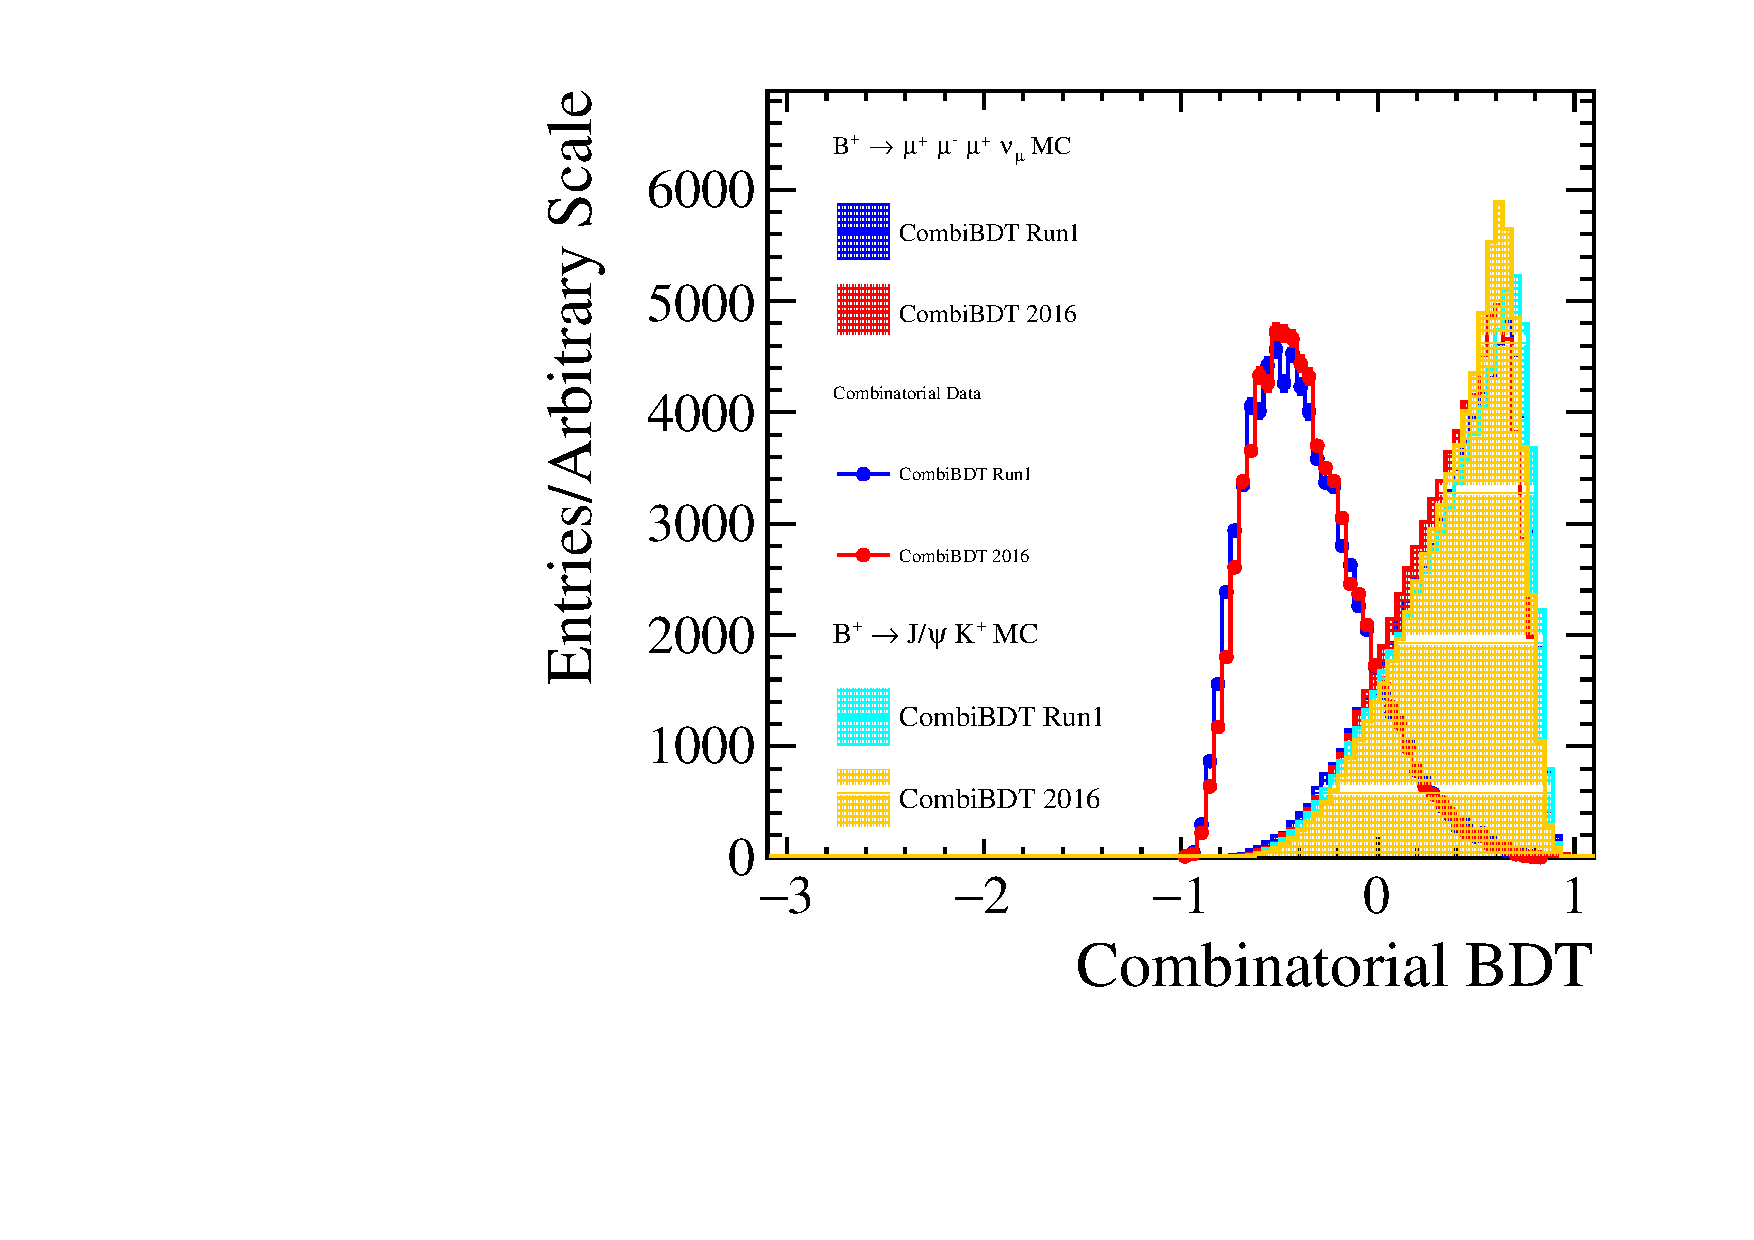
\includegraphics[width = 0.45\textwidth]{efficiency/plot_shapes_before_combibdt_forefficiency/plotvariableCombiBDTNICEFOREFF}\put(-110,133){(a)}%
\includegraphics[width = 0.45\textwidth]{efficiency/plot_shapes_before_combibdt_forefficiency/plotvariableB_PTNICEFOREFF}\put(-110,133){(b)}%
\newline
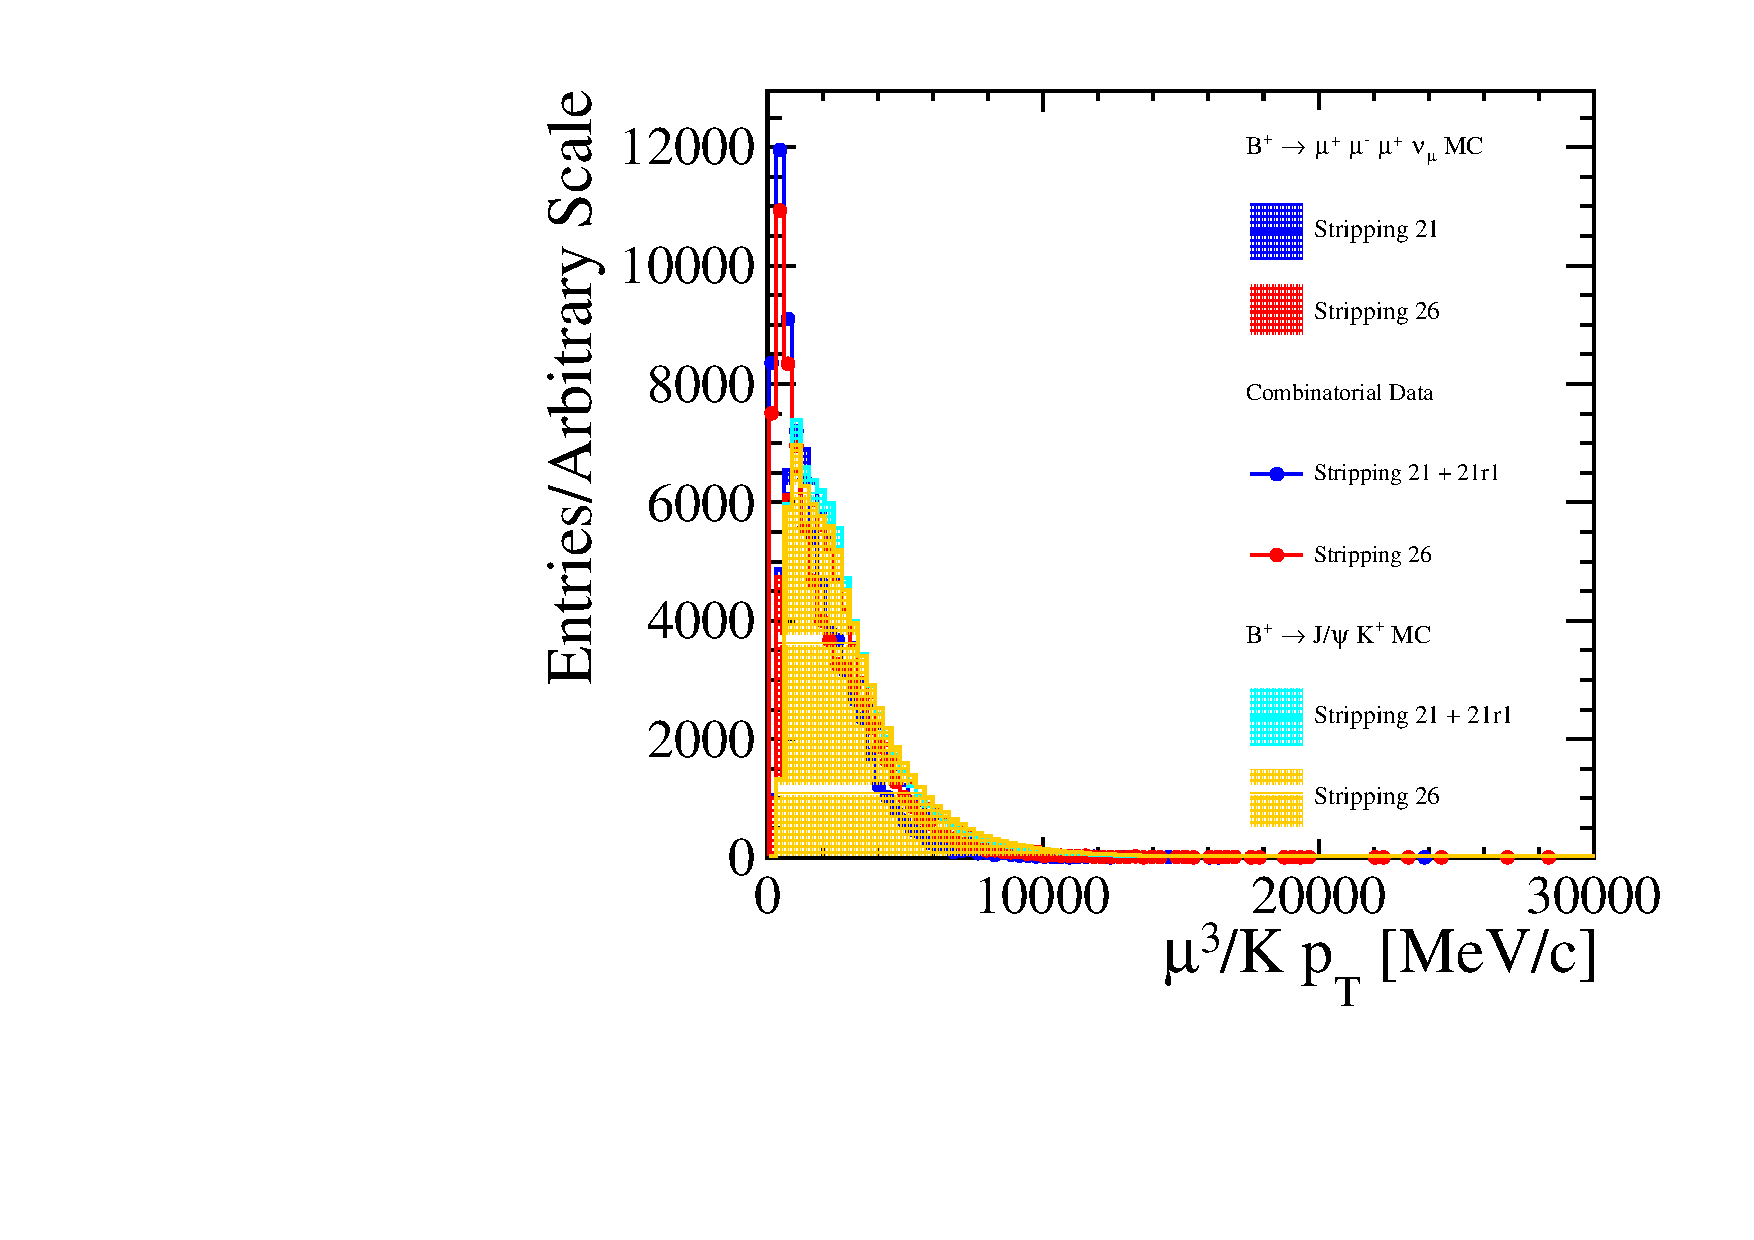
\includegraphics[width = 0.45\textwidth]{efficiency/plot_shapes_before_combibdt_forefficiency/plotvariablemu3_PTNICEFOREFF}\put(-110,133){(c)}%
\includegraphics[width = 0.45\textwidth]{efficiency/plot_shapes_before_combibdt_forefficiency/plotvariablemu3_PNICEFOREFF}\put(-110,133){(d)}%
\caption{(a) Combinatorial BDT response for signal MC and upper mass sideband as well as for normalisation channel MC for Stripping 21 and Stripping 26. The most discriminative variables are (b) $p_{T}$ of B, (c) muon/kaon $p_{T}$ and (d) muon/kaon $p$.}
\label{fig:reason1}
\end{figure}

\begin{figure}[H]
\center
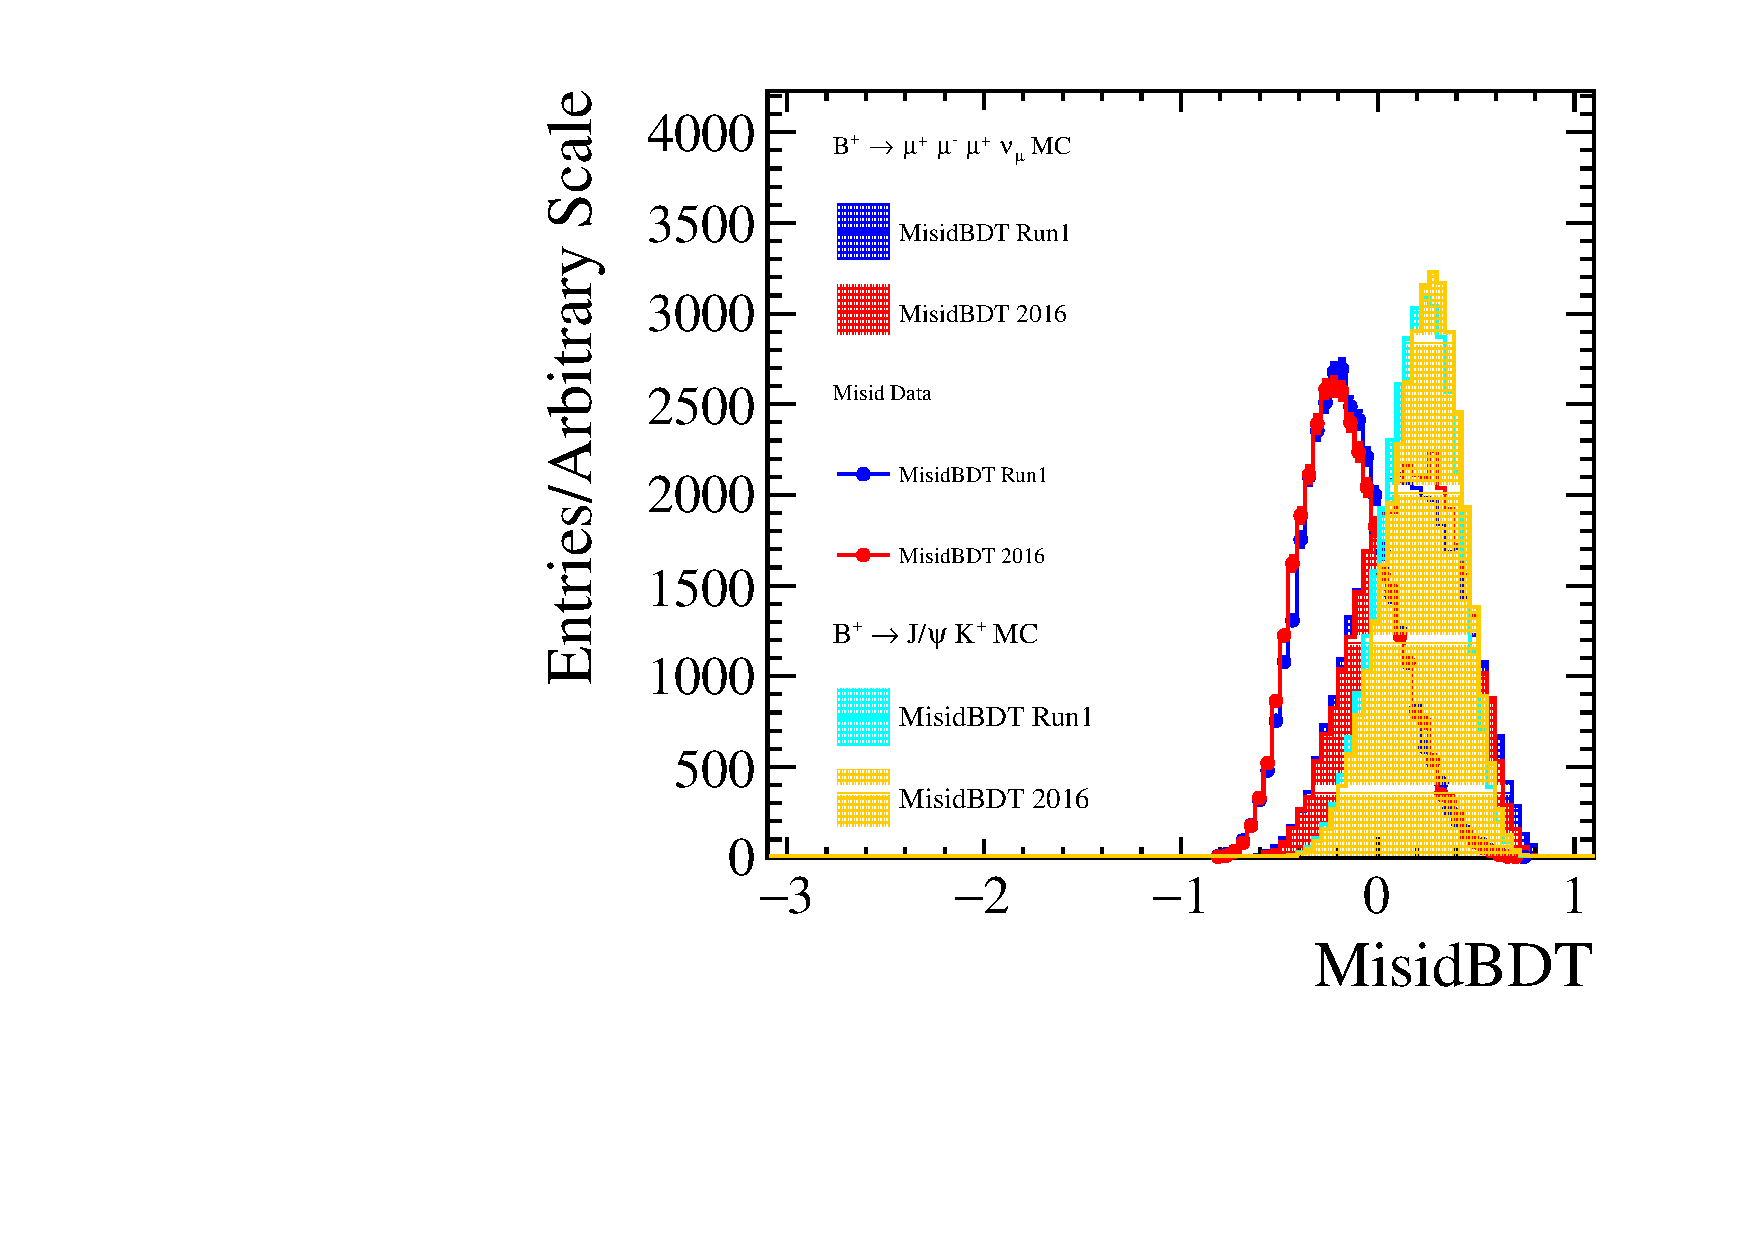
\includegraphics[width = 0.45\textwidth]{efficiency/plot_shapes_before_misidbdt_forefficiency/plotvariableMisidBDTNICEFOREFF}\put(-110,133){(a)}%
\includegraphics[width = 0.45\textwidth]{efficiency/plot_shapes_before_misidbdt_forefficiency/plotvariableB_PTNICEFOREFF}\put(-110,133){(b)}%
\newline
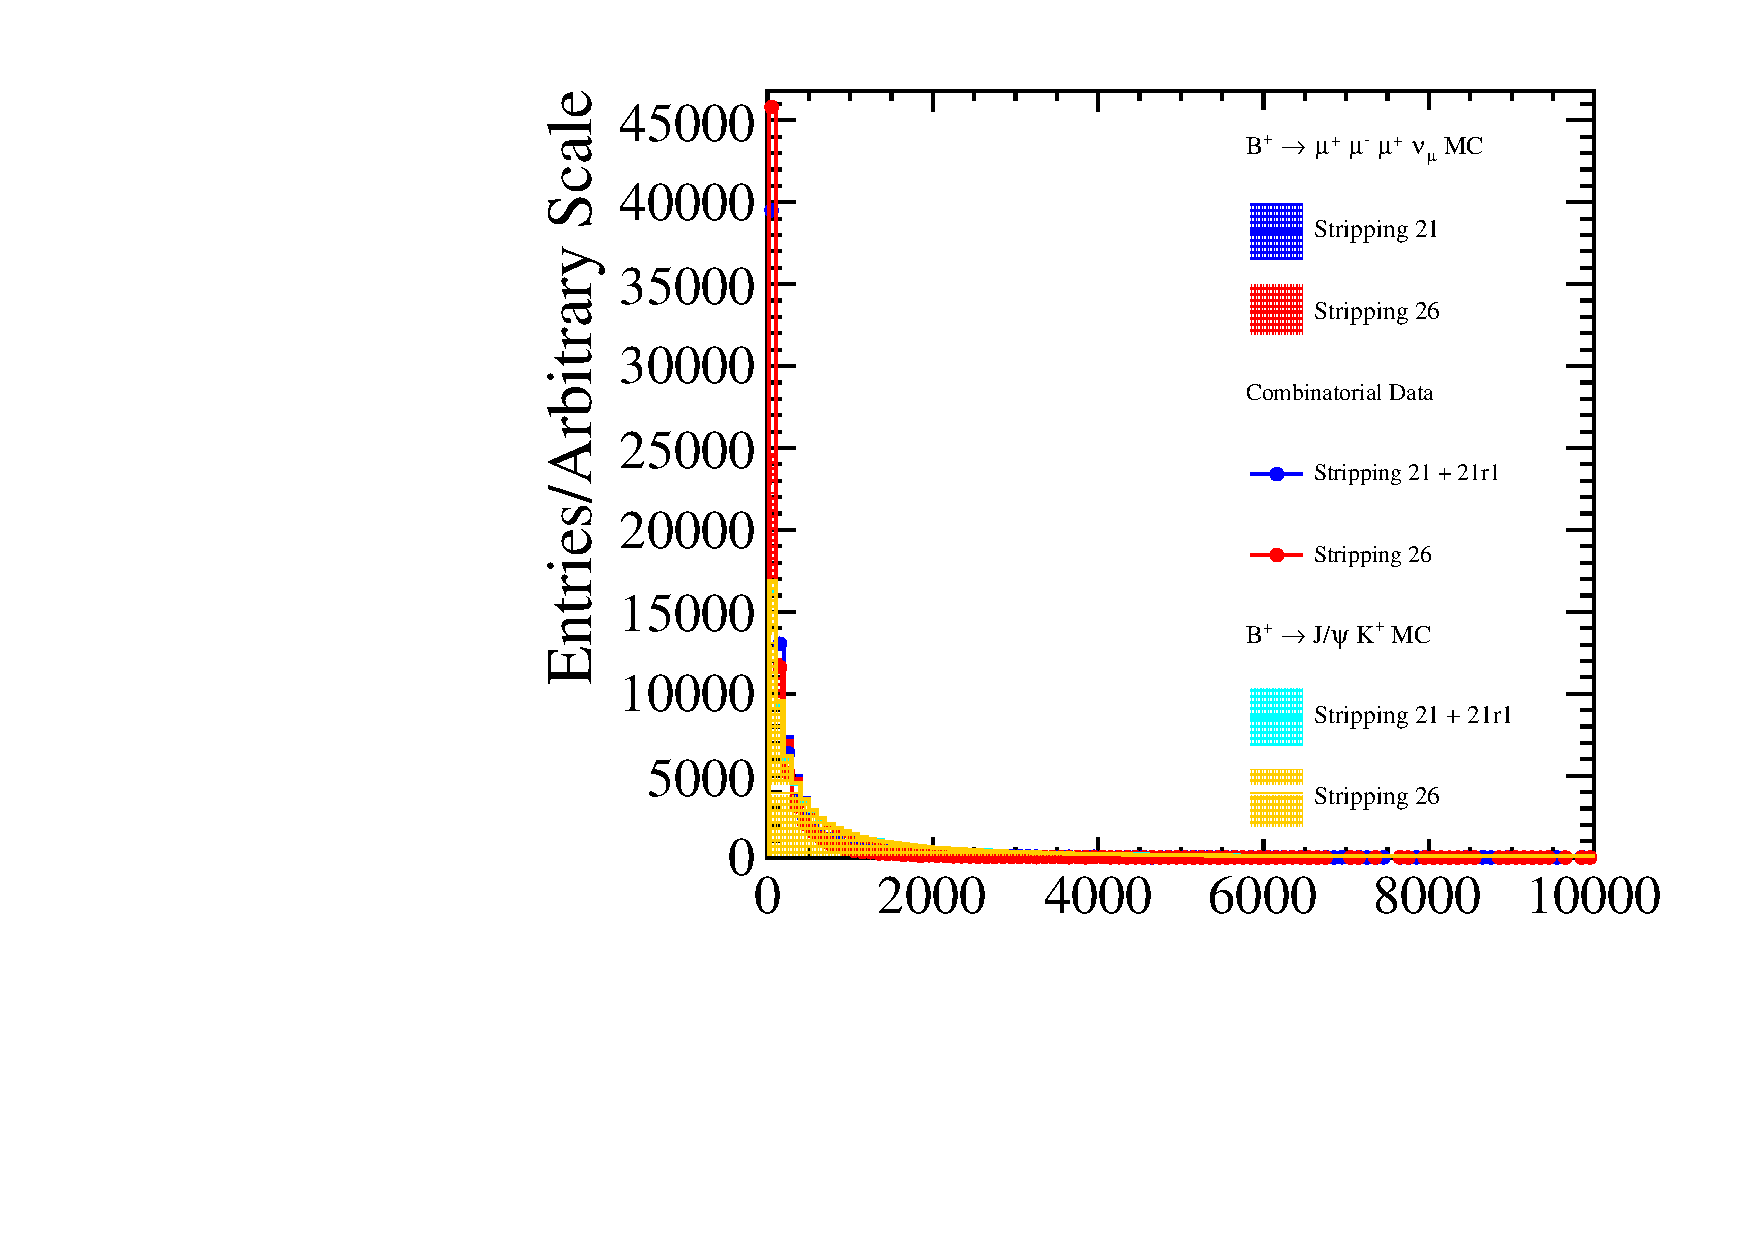
\includegraphics[width = 0.45\textwidth]{efficiency/plot_shapes_before_misidbdt_forefficiency/plotvariablemu2_MINIPCHI2NICEFOREFF}\put(-110,133){(c)}%
\includegraphics[width = 0.45\textwidth]{efficiency/plot_shapes_before_misidbdt_forefficiency/plotvariablemu3_PNICEFOREFF}\put(-110,133){(d)}%
\caption{(a) Misid BDT response for signal MC and upper mass sideband as well as for normalisation channel MC for Stripping 21 and Stripping 26. The most discriminative variables are (b) $p_{T}$ of B, (c) muon IP $\chi^{2}$  and (d) muon/kaon $p$. Misid BDT responses are plotted with combinatorial BDT already applied.}
\label{fig:reason2}
\end{figure}

\subsection{Fitting Range Efficiency (FR)}

As discussed in~\autoref{fittingsel},\mybox{reference combinatorial section}, fitting region was chosen firstly in order to avoid modelling combinatorial background drop in low corrected mass region (exclusion below $4000$ \mevcc) and secondly in order to not include region where there are very few/no events (exclusion above $7000$ \mevcc) in \textbf{corrected mass}. As seen in~\autoref{tab:effsumarry} normalisation channel does not loose many candidates compared to signal channel. This is expected as the \textbf{visible mass} is more constrained in normalisation channel from preselection stage (see ~\autoref{tab:stripcutsBnorm}, where $5150\ \mevcc\ <\ B$ Mass$\ <\ 5450\ \mevcc$) than in signal channel as seen in~\autoref{fig:reasonfitrange}). Hence, restricting region in \textbf{corrected mass} is does not affect normalisation channel much.

\begin{figure}[H]
\center
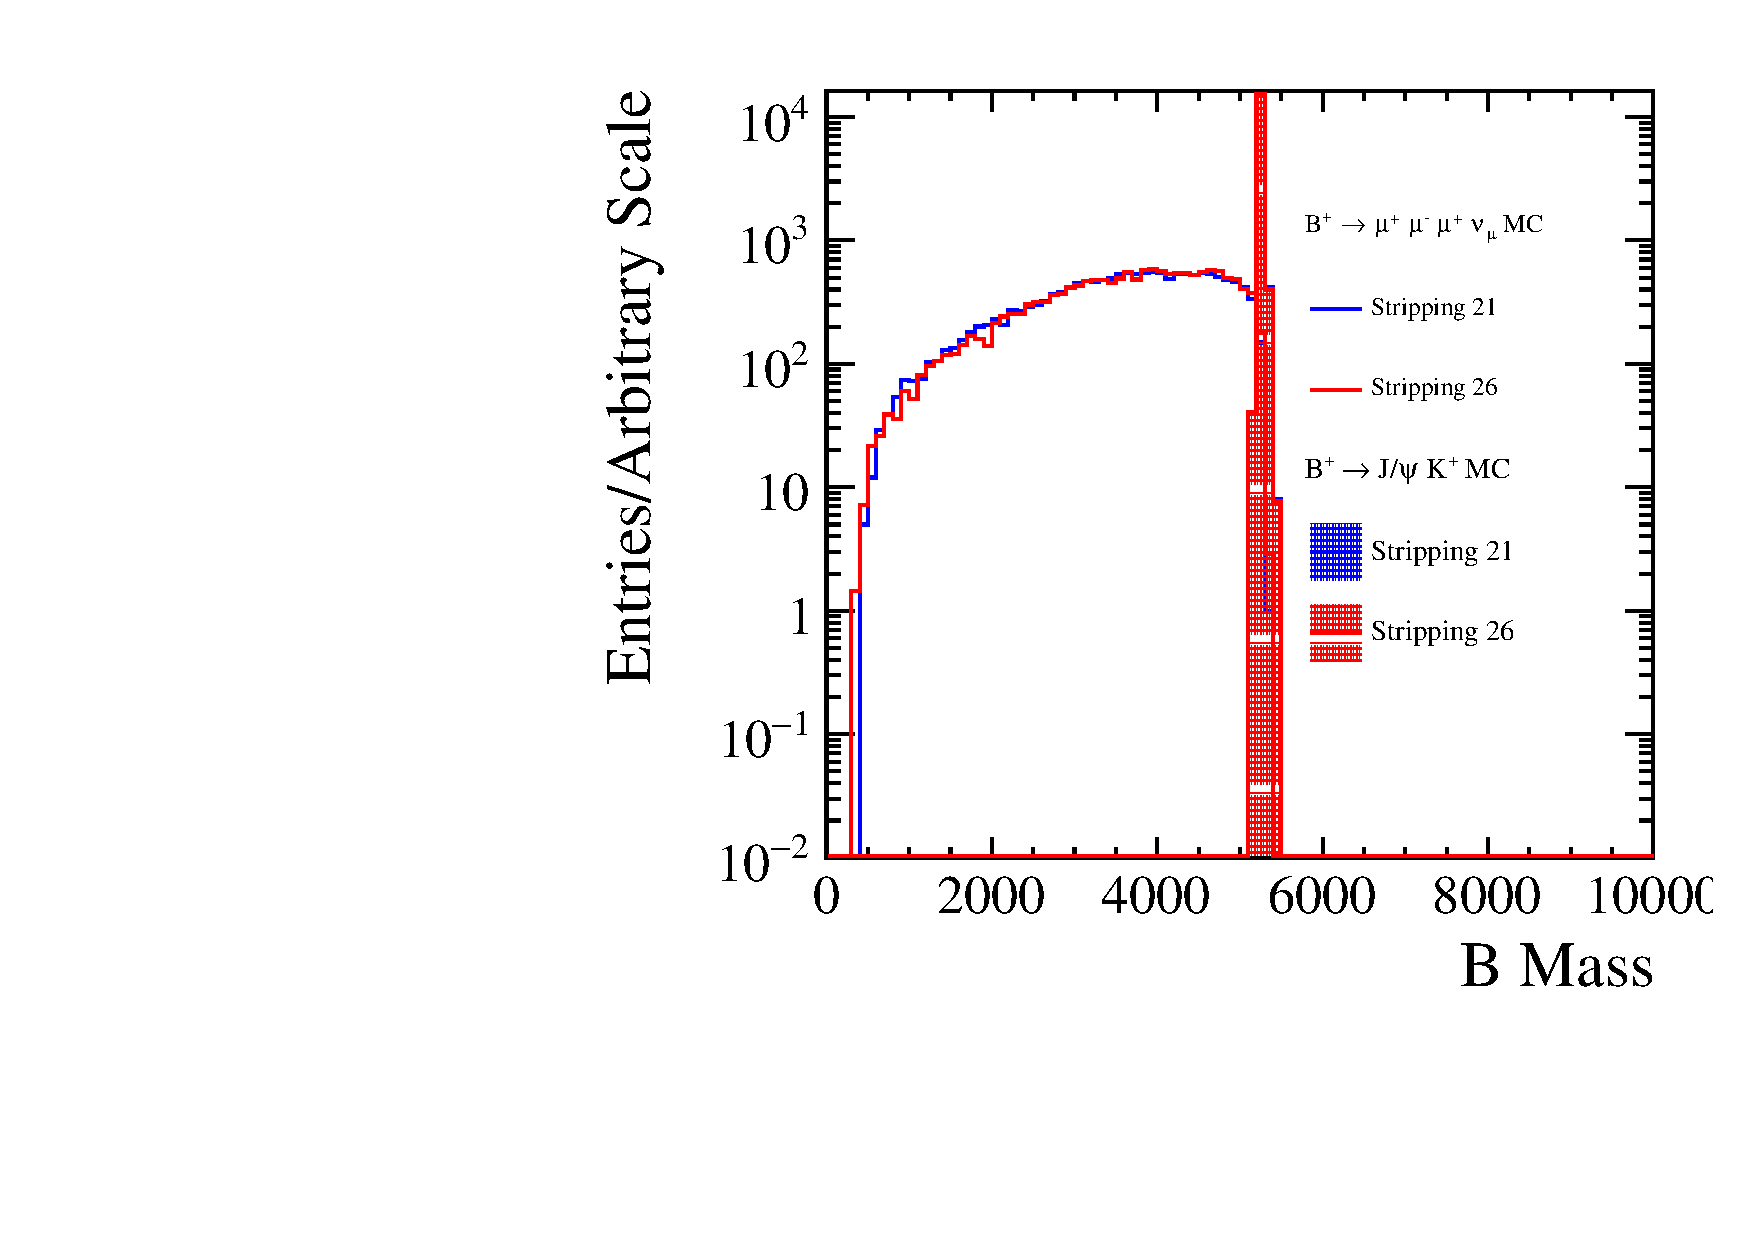
\includegraphics[width = 0.5\textwidth]{efficiency/plot_shapes_fittingregion/plotvariableB_MMMIX.pdf}\put(-110,133){(a)}%
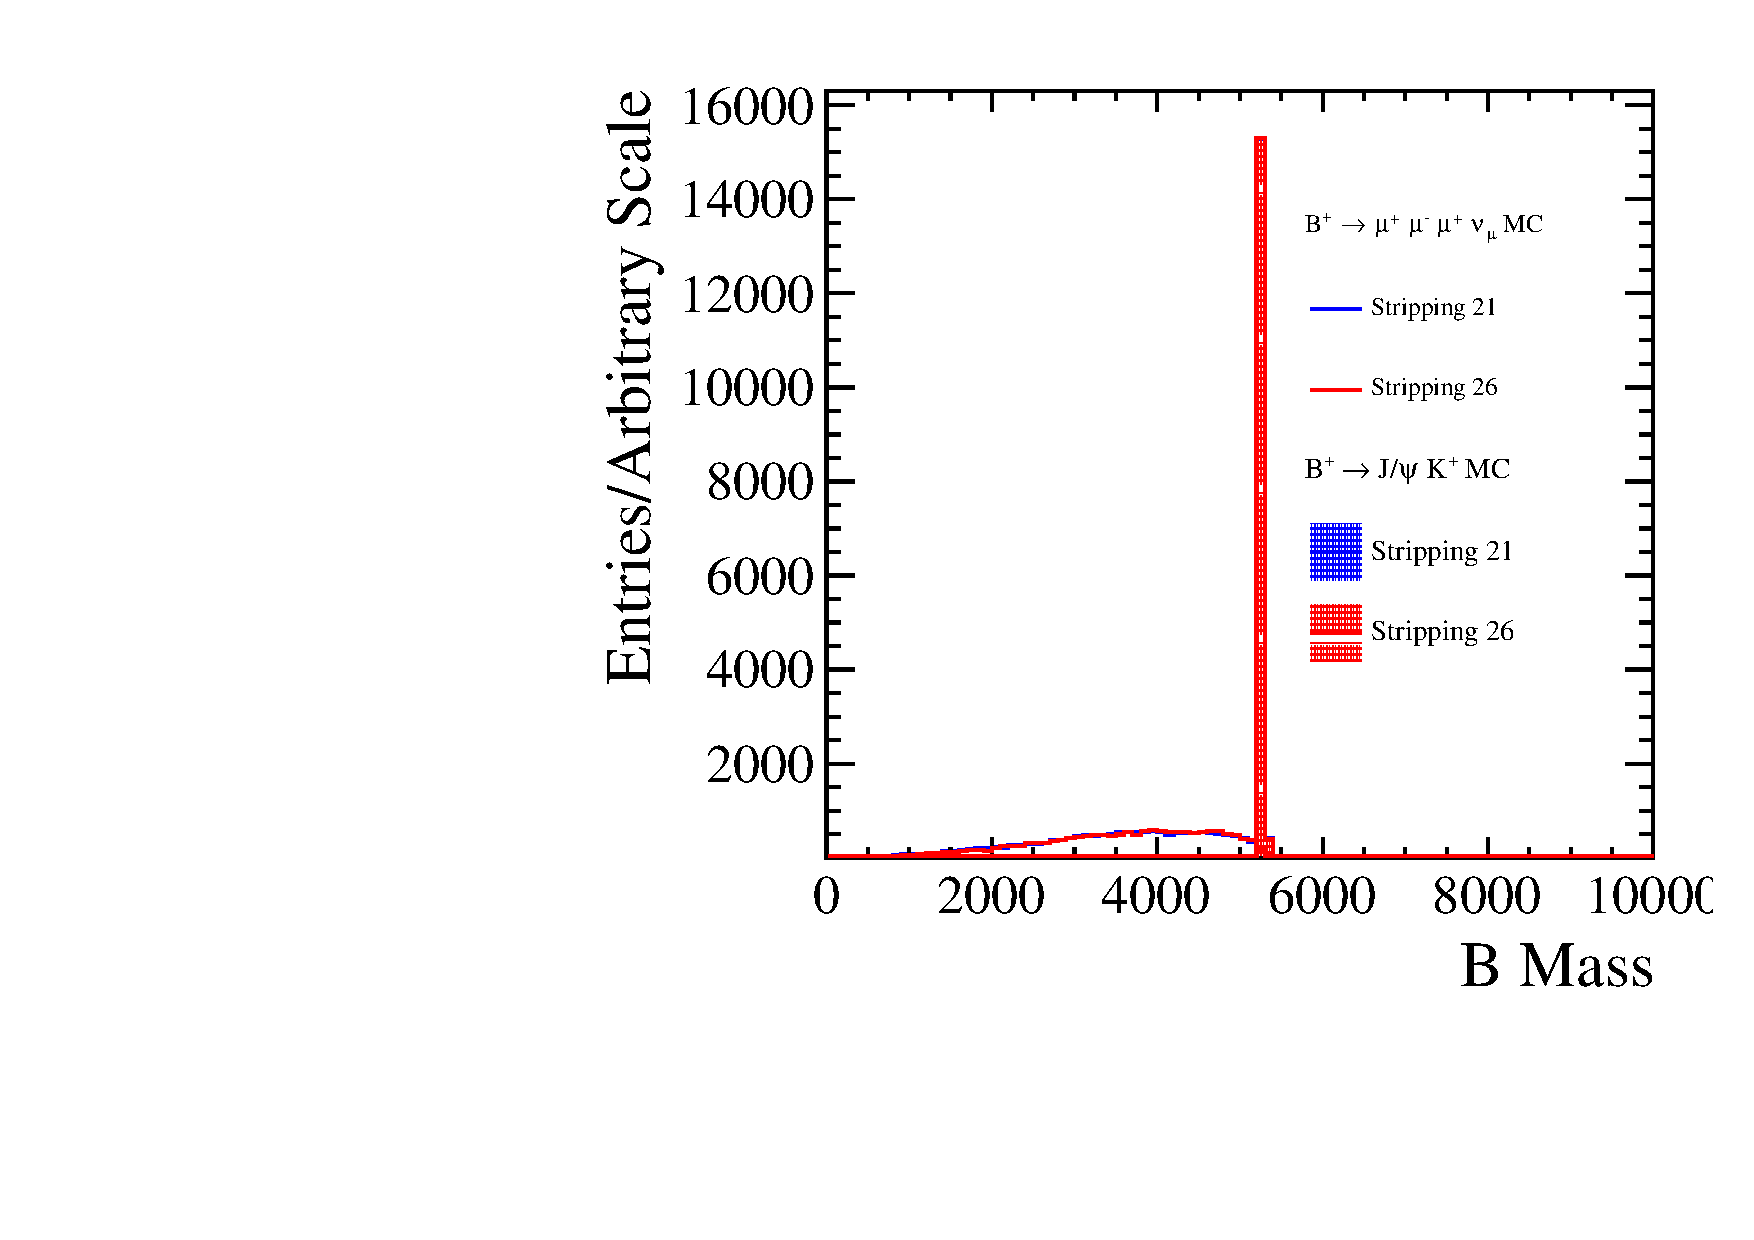
\includegraphics[width = 0.5\textwidth]{efficiency/plot_shapes_fittingregion/plotvariableLogyB_MMMIX.pdf}\put(-110,133){(b)}%
\caption{(a) Visible mass of normalisation and signal simulation. It can be seen that normalisation previous preselection has a sharp cut around $B$ visible mass leading to much higher fitting region efficiency. (b) The corresponding logharitmic version of plot (a).}
\label{fig:reasonfitrange}
\end{figure}


%\begin{table}[H]
%\begin{center}
%\begin{tabular}{ l c  c  c }
%Efficiency & Year &  \Bmumumu  &  \bjpsimumuk \\
%\hline
%$\varepsilon_{FR}$ & 2012  &0.923 & 0.996 \\
%$\varepsilon_{FR}$ & 2016  &0.938 & 0.999 \\
%\hline
%\end{tabular}
%\end{center}
%\caption{Efficiency of fitting range selection.}
%\label{tab:fiteff}
%\end{table}

\subsection{\gls{PID} Efficiencies (PID)}
As \gls{PID} variables are not correctly modelled in simulation, mentioned in~\autoref{simulationchap}, data-driven approach of extracting PID efficiency is taken. To not introduce any biases in previous steps, especially in multivariate selection, PID efficiencies are evaluated at the end of the selection chain with \texttt{PIDCalib} package data samples.

The PID efficiency is higher for normalisation channel with all PID requiremnts givne in~\autoref{tab:PIDselectionNorm} compared to signal provided in~\autoref{tab:PIDselection} due to weaker PID requirement on kaon as compared to muons.

\begin{table}[H]
\begin{center}
\begin{tabular}{l c c}

%    \begin{tabular}{ | l | c | } %p{7cm}|}
    species  & 2012 PID Simulation & 2016 PID Simulation\\ \hline
    muon &  $\Delta LL(\mu - \pi) > 0$ & $\Delta LL(\mu - \pi) > 0$ \\
    muon &  $\Delta LL(\mu - K) > 0$ & $\Delta LL(\mu - K) > 0$ \\
    muon &   - & \texttt{IsMuonTight==1.0}\\
    muon &  \texttt{Nshared==0} & \texttt{Nshared<2} \\
	muon &  \texttt{Probnnmu}$>0.35$ & \texttt{Probnnmu}$>0.35$ \\
     \hline
   $\varepsilon_{PID}$   & 0.631$\pm$ 0.005 & 0.623$\pm$0.006 \\

     \hline
      \end{tabular}

\end{center}
\caption{Signal simulation efficiency using \texttt{PIDCalib} efficiencies.}
\label{tab:PIDselection}
\end{table}

\begin{table}[H]
\begin{center}
\begin{tabular}{l c c}

%    \begin{tabular}{ | l | c | } %p{7cm}|}
    species  &2012 PID Simulation & 2016 PID Simulation\\ \hline
    muon &  $\Delta LL(\mu - \pi) > 0$ & $\Delta LL(\mu - \pi) > 0$ \\
    muon & $\Delta LL(\mu - K) > 0$ & $\Delta LL(\mu - K) > 0$ \\
    muon &  - & \texttt{IsMuonTight==1.0}\\
    muon & \texttt{Nshared==0} & \texttt{Nshared<2} \\
    muon & \texttt{Probnnmu}$>0.35$ & \texttt{Probnnmu}$>0.35$ \\
    kaon &  $\Delta LL(K - \pi) > 0$ & $\Delta LL(K - \pi) > 0$ \\
    kaon &  $\Delta LL(p - K) < 5$ & $\Delta LL(p - K) < 5$ \\
     \hline
    $\varepsilon_{PID}$ &0.685$\pm$ 0.001 & 0.656$\pm$0.001  \\

     \hline
      \end{tabular}

\end{center}
\caption{Normalisation MC efficiency using \texttt{PIDCalib} efficiencies.}
\label{tab:PIDselectionNorm}
\end{table}


%\section{Summary of efficiencies}
%\label{EfficiencySummary}
%
%The summary of individual efficiencies together with total efficiency, which is calculated for signal using nominator of \autoref{eq:notsplitted} and for normalisation denominator of \autoref{eq:notsplitted}, is given in \autoref{tab:effsumarry}.
%%taken from /vols/lhcb/ss4314/tablesforana/efficiencyratios/2016/SesFUMSB_NOTsimultaneous_full_Error/plot_interesting/bin/*OK*per*tex
%\begin{table}[H]
%\begin{center}
%\medskip
%\begin{tabular}{ 
%  l|  
%  >{\collectcell\num}r<{\endcollectcell}@{${}\pm{}$}>{\collectcell\num}l<{\endcollectcell} 
%  >{\collectcell\num}r<{\endcollectcell}@{${}\pm{}$}>{\collectcell\num}l<{\endcollectcell} |
%  >{\collectcell\num}r<{\endcollectcell}@{${}\pm{}$}>{\collectcell\num}l<{\endcollectcell}
%  >{\collectcell\num}r<{\endcollectcell}@{${}\pm{}$}>{\collectcell\num}l<{\endcollectcell}
%  }	
%%\toprule
%
%
%        \hline
%\multicolumn{1}{l|}{} & \multicolumn{4}{c|}{$ B^{+} \rightarrow \mu^{+} \mu^{-} \mu^{+} \nu$} & \multicolumn{4}{c}{$B^{+} \rightarrow (J/\psi \rightarrow \mu^{+} \mu^{-}) K^{+}$} \\
%	Efficiency & \multicolumn{2}{c}{2012} & \multicolumn{2}{c|}{2016} & \multicolumn{2}{c}{2012} & \multicolumn{2}{c}{2016} \\
%
%%\midrule
%
%        \hline
%
%$\varepsilon_{GEN}$ & 18.56& 0.11 & 19.59& 0.07 & 16.22& 0.02 & 17.39& 0.02 \\
%$\varepsilon_{REC}$ & 10.84& 0.03 & 12.40& 0.01 & 17.74& 0.01 & 20.03& 0.00 \\
%$\varepsilon_{TRG}$ & 74.22& 0.13 & 74.83& 0.05 & 77.79& 0.03 & 79.12& 0.01 \\
%$\varepsilon_{OFF}$ & 88.20& 0.11 & 88.30& 0.05 & 100.00& 0.00 & 100.00& 0.00 \\
%$\varepsilon_{CombiBDT}$ & 47.25& 0.18 & 34.28& 0.07 & 50.89& 0.05 & 39.73& 0.02 \\
%$\varepsilon_{MisidBDT}$ & 43.58& 0.26 & 36.80& 0.12 & 51.12& 0.07 & 44.64& 0.02 \\
%$\varepsilon_{FR}$ & 92.30& 0.21 & 93.77& 0.10 & 99.59& 0.01 & 99.91& 0.00 \\
%$\varepsilon_{PID}$ & 63.15& 0.50 & 62.27& 0.27 & 68.53& 0.11 & 65.63& 0.04 \\
%\hline
%
%$\varepsilon_{total}$ & 0.1581& 0.0020 & 0.1182& 0.0008 & 0.3974& 0.0011 & 0.3203& 0.0005 \\
%
%	
%	
%	\hline
%%\bottomrule
%\end{tabular}
%\end{center}
%\caption{Summary of individual simulation and/or data efficiencies in \% necessary for \textit{single event sensitivity} for signal and normalisation channel. Efficiency values for 2016 are TCK-weighted averaged efficiencies. The errors considered are of statistical nature, computed using binomial error.}
%\label{tab:effsumarry}
%\end{table}
%
%
%Hence resulting values for relative no fractional corrected mass split efficiency ratios defined in \autoref{eq:notsplitted} are
%
%\begin{equation}
%	R^{21}_{\rm{NOFCME}}(\varepsilon)=\frac{(1.58\pm0.02)\times 10 ^{-3 }}{(3.97\pm0.01)\times 10 ^{-3 }}=(3.98\pm0.05)\times 10 ^{-1 },
%\end{equation}
%
%\begin{equation}
%	R^{26}_{\rm{NOFCME}}(\varepsilon)=\frac{(1.18\pm0.01)\times 10 ^{-3 }}{(3.20\pm0.00)\times 10 ^{-3 }}=(3.69\pm0.03)\times 10 ^{-1 }.
%\end{equation}
%
%
%Including fractional corrected mass split efficiency ratios defined in~\autoref{eq:impsplit}
%
%\begin{equation}
%	R^{21}_{\rm{lowFCME}}(\varepsilon)=\frac{(7.44\pm0.12)\times 10 ^{-4 }}{(2.33\pm0.01)\times 10 ^{-3 }}=(3.20\pm0.05)\times 10 ^{-1 },
%\end{equation}
%\begin{equation}
%	R^{21}_{\rm{highFCME}}(\varepsilon)=\frac{(8.37\pm0.13)\times 10 ^{-4 }}{(1.65\pm0.01)\times 10 ^{-3 }}=(5.09\pm0.08)\times 10 ^{-1 },
%\end{equation}
%
%\begin{equation}
%	R^{26}_{\rm{lowFCME}}(\varepsilon)=\frac{(6.51\pm0.05)\times 10 ^{-4 }}{(2.15\pm0.00)\times 10 ^{-3 }}=(3.03\pm0.02)\times 10 ^{-1 },
%\end{equation}
%\begin{equation}
%	R^{26}_{\rm{highFCME}}(\varepsilon)=\frac{(5.33\pm0.05)\times 10 ^{-4 }}{(1.05\pm0.00)\times 10 ^{-3 }}=(5.06\pm0.04)\times 10 ^{-1 }.
%\end{equation}
%	
%	
%As it can be noticed, different selections that were optimised for Run \Rn{1} and \Rn{2} yield different overall as well as individual efficiencies. This results in small differences in sensitivity between Run \Rn{1} and Run \Rn{2}. To better understand where does this difference come from, ratio of individual relative efficiencies as a function of stripping version is plotted in the~\autoref{fig:rateffsnofcme}. The difference can be attributed to different BDTs.
%
%\begin{figure}[H]
%\centering
%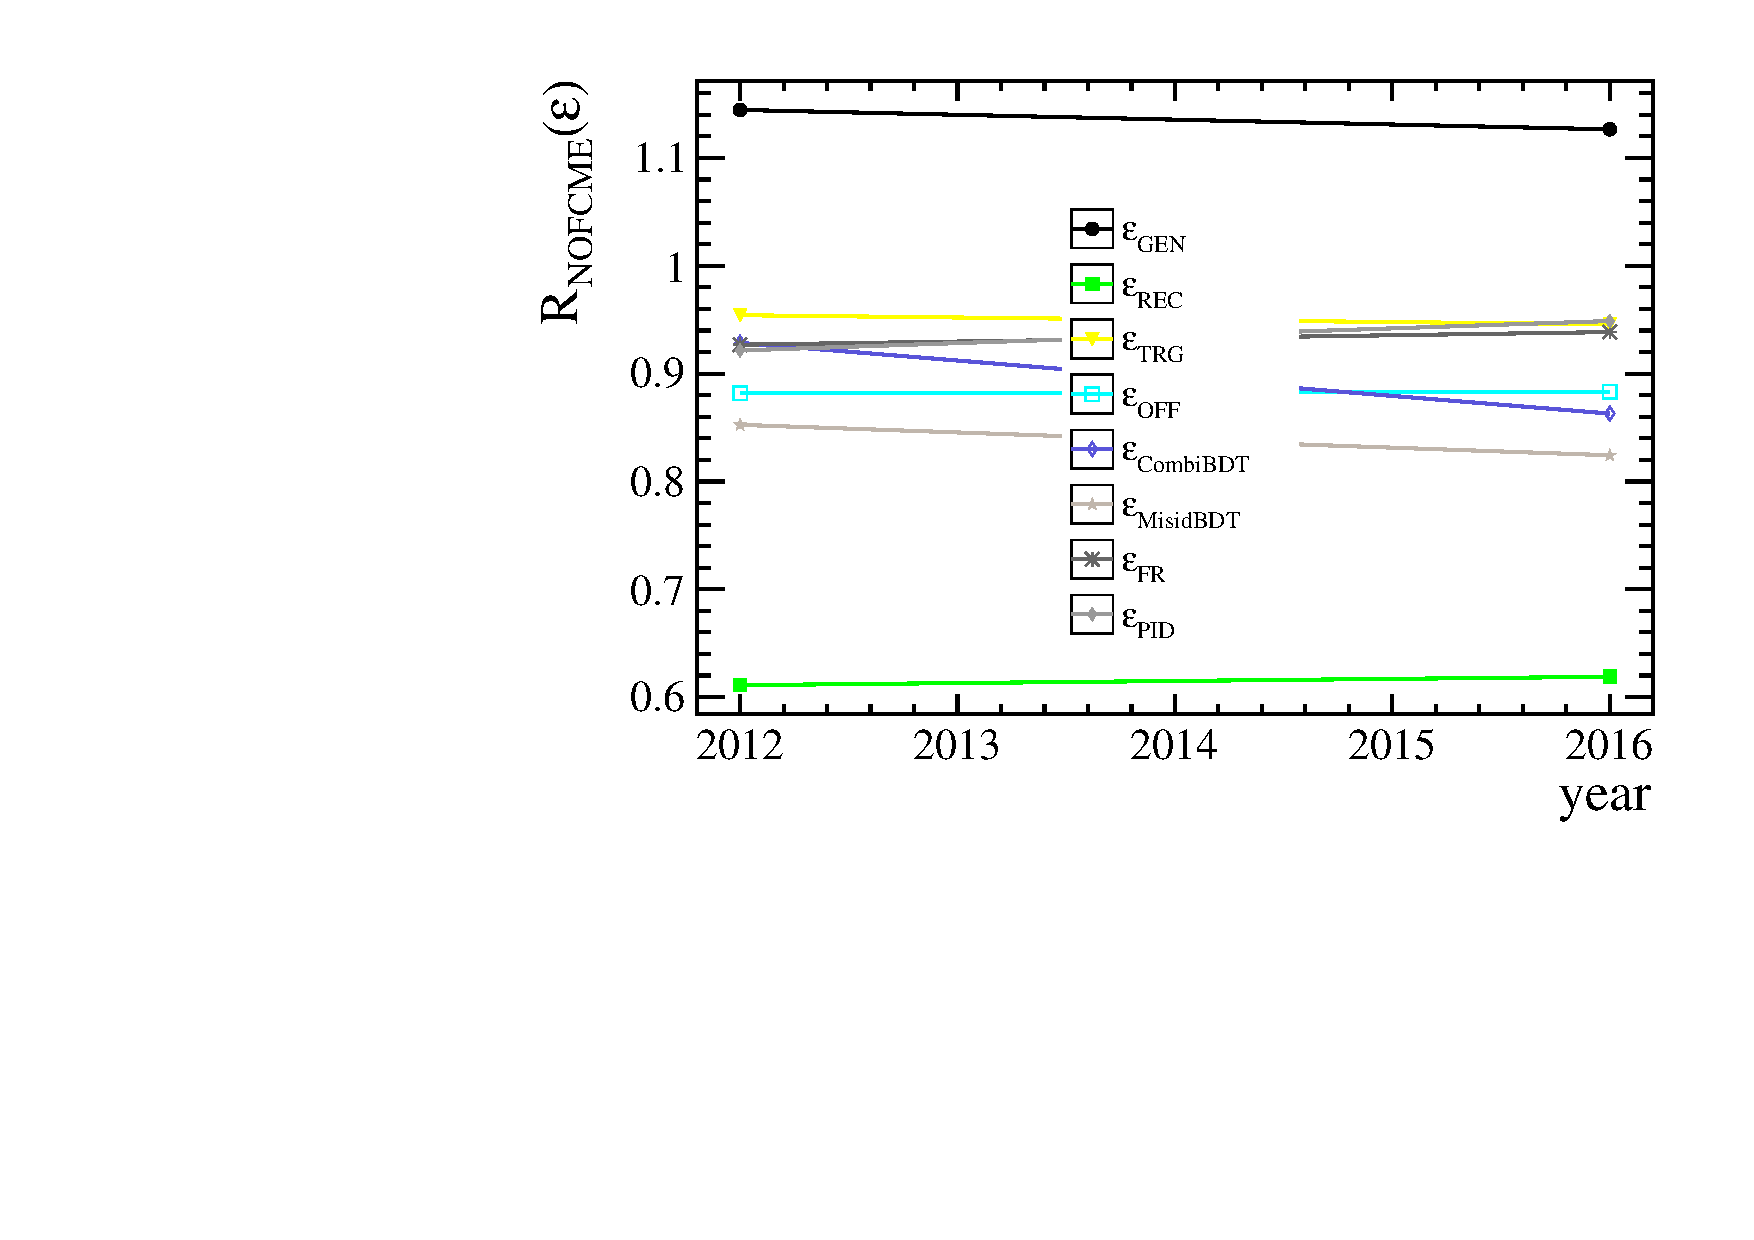
\includegraphics[width = 0.8\textwidth]{efficiency/effiratio/Plot_ALL_Efficiencies_Ratio_Overview_Pretty.pdf}
%\caption{Summary of ratio of efficiencies between 2012 simulation and 2016 simulation with no FCME split. Efficiency values for 2016 are TCK-weighted averaged efficiencies.}
%\centering
%\label{fig:rateffsnofcme}
%\end{figure}



%\begin{table}[H]
%\begin{center}
%\begin{tabular}{ l  c  c  c  c  }
%\multicolumn{1}{ l }{} & \multicolumn{2}{c}{Low FCME} & \multicolumn{2}{c}{High FCME} \\
%Efficiency & 2012 & 2016 & 2012 & 2016 \\
%\hline
%$\varepsilon_{dec^{s}}$ & 0.186 & 0.196 & 0.186 & 0.196 \\
%$\varepsilon_{dec^{n}}$ & 0.162 & 0.174 & 0.162 & 0.174 \\
%$\varepsilon_{rec^{s}}$ & 0.108 & 0.124 & 0.108 & 0.124 \\
%$\varepsilon_{rec^{n}}$ & 0.177 & 0.2 & 0.177 & 0.2 \\
%$\varepsilon_{trg^{s}}$ & 0.742 & 0.748 & 0.742 & 0.748 \\
%$\varepsilon_{trg^{n}}$ & 0.778 & 0.791 & 0.778 & 0.791 \\
%$\varepsilon_{off^{s}}$ & 0.882 & 0.883 & 0.882 & 0.883 \\
%$\varepsilon_{off^{n}}$ & 1 & 1 & 1 & 1 \\
%$\varepsilon_{combi^{s}}$ & 0.473 & 0.343 & 0.473 & 0.343 \\
%$\varepsilon_{combi^{n}}$ & 0.509 & 0.397 & 0.509 & 0.397 \\
%$\varepsilon_{misid^{s}}$ & 0.436 & 0.368 & 0.436 & 0.368 \\
%$\varepsilon_{misid^{n}}$ & 0.511 & 0.446 & 0.511 & 0.446 \\
%$\varepsilon_{corm^{s}}$ & 0.923 & 0.938 & 0.923 & 0.938 \\
%$\varepsilon_{corm^{n}}$ & 0.996 & 0.999 & 0.996 & 0.999 \\
%$\varepsilon_{FCME^{s}}$ & 0.484 & 0.548 & 0.516 & 0.452 \\
%$\varepsilon_{FCME^{n}}$ & 0.593 & 0.673 & 0.407 & 0.327 \\
%$\varepsilon_{pid^{s}}$ & 0.615 & 0.625 & 0.647 & 0.62 \\
%$\varepsilon_{pid^{n}}$ & 0.677 & 0.654 & 0.697 & 0.661 \\
%\hline
%\end{tabular}
%\end{center}
%\caption{Summary of individual simulation and/or data efficiencies necessary for \textit{Single Event Sensitivity} for signal (\textit{s}) and normalisation channel (\textit{n}) with FCME split. Efficiency values for 2016 are TCK-weighted averaged efficiencies.}
%\label{tab:effsfcme}
%\end{table}

